\chapterimage{Fig/Chapter1/cover.png}

\chapter{Quantum correlations in the weakly-interacting Bose gas}

\label{sec:chapter_1}

\fancyhead[LO]{\rightmark} % Print the nearest section name on the left side of odd pages
\fancyhead[RE]{\leftmark}



% One of the key and on-going challenges of quantum mechanics is to understand macroscopic systems containing a large number of particles $N$, commonly referred as many-body physics. Trying to consider all the possible degrees of freedom of each individual particle and interactions effects would result in an incredibly complex problem impossible to solve theoretically. Studying such systems thus require to use approximations ...

% Physicists were able to describe a gas of a large number of bosonic particles with increasing complexity throughout history. The first step was the development of statistical physics, aiming to build a bridge between the microscopic properties of individual atoms or molecules and macroscopic properties of bulk materials described by thermodynamics. This approach culminated in the theory of the ideal Bose gas, ideal meaning here that all particles are non-interacting. This theory found great success with the notable prediction of a new state of matter, the Bose-Einstein condensate. 

% The next step was then to increase the complexity of the problem by adding interactions between the particles. ...

% While also greatly successful, the mean-field approach neglects by essence interaction phenomena between individual particles. To characterize such effects, we thus need to go beyond the mean-field approximation. ...

The main challenge of quantum many-body physics is to understand how ensembles of interacting individual particles behave. Towards this aim, many meaningful information can be obtained by studying how the interactions between the different particles induce \textbf{correlations} in the degrees of freedom of the particles, {\it e.g.} their position, their momentum or their spin. To understand and quantify these correlations, physicists have used the mathematical formalism of \textbf{correlation functions} that we will introduce in this chapter. 

Historically, the first field of physics that developed and made an extensive use of correlation functions was the field of Optics, and more specifically Quantum Optics in the 50s-60s. The interest for correlation functions was sparked by the Hanbury Brown and Twiss experiment of 1954 measuring intensity correlations in the light emitted by a star between two separate photo-detectors. Trying to provide an explanation of these experiments in terms of the detection of individual photons led R. J. Glauber to develop his theory of photodetection \cite{glauber1963quantum} using correlation functions in a seminal paper of 1963. This theory was then later adapted to study more complex systems where the particles, for instance atoms, interact. 

One of the conceptually simplest example of such an interacting many-body system is the weakly-interacting homogeneous Bose gas, which describes an ensemble of bosons with weak contact and repulsive interactions in an homogeneous box potential. This system shows the great advantage that it can be theoretically described with a fairly great accuracy at the price of a few approximations that were suggested by N. Bogoliubov in 1947 \cite{bogoliubov1947}. One of the great success of this theory was to predict the existence of the quantum depletion that was later showed to be made of \kmk correlated pair of atoms by Lee Huang and Yang \cite{lee1957} in 1957.

An experimental realisation of such a system proves to be rather difficult because of the \textbf{homogeneous} aspect of the theory that is hard to reproduce experimentally. Only recently were Bose gases realized in box traps in Cambridge \cite{gaunt2013bose} and the quantum depletion studied in this homogeneous configuration \cite{lopes2017}. But experiments often rely on an harmonic potential to trap the atoms in one place, therefore breaking the homogeneity of the system and making theoretical approaches more complicated. However, recent works \cite{butera2020,mathey2009noise,toth2008theory} have aimed at characterizing correlation functions within the frame of Bogoliubov theory for inhomogeneous trapped systems to provide theoretical ground for comparison with experiments. 

In this chapter, we will first introduce the concept of correlation functions by studying the historical and founding experiments of Optics and Quantum Optics. In a second stage, we will show how this formalism can be extended to atomic physics and apply it to the Bogoliubov theory of the homogeneous weakly-interacting Bose gas of which we will present the main lines. Finally, we will present some of the principal results of the work \cite{butera2020} extending the Bogoliubov theory to inhomogeneous systems produced with our experiment and discuss the experimental criteria to experimentally observe the \kmk correlations of the quantum depletion. 




\section{Correlation functions in Classical and Quantum Optics}

In the most general sense, correlation functions are a mathematical object characterizing the statistical correlations between random variables. They are defined from the concept of statistical average or expected value of a random variable in Mathematics which is intuitively understood as the value that we will get on average if we measure the random variable a large number of occurences. In the following, the statistical average of a random variable $X$ is denoted $\mean{X}$.

The simplest correlation function correlating two random variables $X_1$ and $X_2$ that we take to be real for this simple introduction writes:

\begin{equation}
    \text{Corr}(X_1,X_2)=\mean{X_1 X_2}
\end{equation}

\noindent Interestingly, if $X_1$ and $X_2$ are independent and therefore uncorrelated, one has:

\begin{equation}
    \mean{X_1 X_2} = \mean{X_1} \mean{X_2}
    \label{eq:indep_variables}
\end{equation}

\noindent meaning that the expected value of the product $X_1 X_2$ is simply the product of the expected values of $X_1$ and $X_2$. However, if $X_1$ and $X_2$ are correlated, the probability distribution of $X_2$ changes if we already know the realisation of $X_1$, preventing us to write the simple equation \ref{eq:indep_variables}. The value of $\mean{X_1 X_2}$ thus quantifies the degree of correlation of the two random variables. The concept of correlation function can be generalized up to any order to involve several random variables. We also note that in physics, the random variables are often dependent from time, space etc.. In all generality, the correlation function correlating $n$ random variables writes:

\begin{equation}
    \text{Corr}^{(n)}(X_1(s_1),X_2(s_2),...,X_i(s_i),...,X_n(s_n)) = \mean{X_1(s_1) X_2(s_2) ... X_i(s_i) ... X_n(s_n)} 
\end{equation}
\noindent where $s_i$ is the proper set of parameters describing the variable $X_i$.

\subsection{First order correlation function of classical light}

Having seen the general definition of correlation functions, let us now illustrate how they can be used in Physics with the simple example of the classical description of light. Correlation functions of light were introduced in connection with the notion of \textbf{coherence} that characterizes the possibility for waves to interfere. A light field is said to be coherent when there is a fixed phase relationship for the electric field at different positions (spatial coherence) and different times (time coherence). 


\begin{figure}
    \centering
    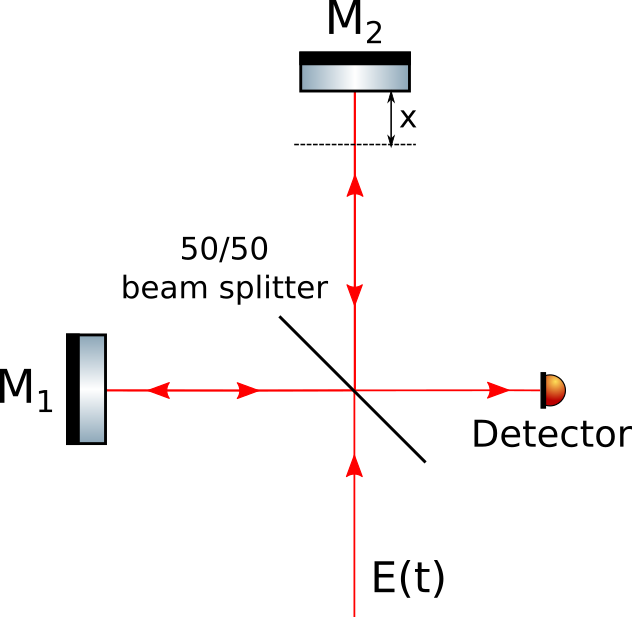
\includegraphics[width=0.55\textwidth]{Fig/Chapter1/michelson.png}
    \caption{Principle of the Michelson interferometer.}
    \label{fig:michelson}
\end{figure}


To illustrate where correlation functions come from, we will first look at time coherence in the emblematic Michelson interferometer (see Fig.-\ref{fig:michelson}). For simplicity sake, we will not yet discuss spatial coherence effects and will thus consider a point source producing a complex, linearly-polarized light field $E(t)$ that enters the interferometer. The intensity measured by the detector writes\footnote{While we write here an equal sign for clarity, we strictly speaking only have $I \propto \mean{\abs{E(t)+E(t-\tau)}^2}$}:

\begin{equation}
    I= \langle \lvert E(t)+E(t-\tau)\lvert^2 \rangle
    \label{eq:i_michelson}
\end{equation}

\noindent with $\tau=\frac{2x}{c}$ the delay between the two interfering waves induced by the optical path difference between the two arms of the interferometer. Developing equation \ref{eq:i_michelson} we get:

\begin{equation}
    I=\mean{\abs{E(t)}^2}  + \mean{E(t-\tau)^2} + 2 {\rm{Re}} \mean{E(t) E^*(t-\tau)}
    \label{eq:def_g1}
\end{equation}

For simplicity sake, we assume that the source is stationary to write $\mean{\abs{E(t)}^2} = \mean{\abs{E(t-\tau)}^2} = I_0$, we then obtain :

\begin{equation}
    I= 2 I_0 \Big(1 + {\rm{Re}} \Big[g^{(1)} (\tau) \Big] \Big) \ , \ g^{(1)} (\tau) = \frac{ \mean{E(t) E^*(t-\tau)}}{\mean{\abs{E}^2}}
\end{equation}

\noindent We have introduced the \textbf{normalized first-order correlation function} $g^{(1)}$ that characterizes the interference term. If $E(t)$ and $E(t-\tau)$ are independent random variables and thus uncorrelated, $\mean{E(t) E^*(t-\tau)} = \mean{E(t)} \mean{ E^*(t-\tau)}=0$ and interference are not observed. On the other hand, if there is a \textbf{correlation} between these two quantities, an interference phenomenon can be observed. 

To illustrate what kind of information are contained in this first-order correlation function, we compute it for the simple case of a monochromatic light source of frequency $\omega_0$. The light field writes:

\begin{equation}
    E(t)=E_0 e^{i \omega_0 t}
\end{equation}

\noindent Such a light source is perfectly coherent. From this, we calculate the first-order correlation function:

\begin{equation}
    g^{(1)} (\tau) = \frac{|E_0|^2 \mean{e^{i\omega_0 t} e^{-i \omega_0 (t-\tau)}}}{|E_0|^2} = e^{i \omega_0 \tau}
\end{equation}

\noindent The detected intensity is thus a perfect sinusoidal function of $\tau$ that is scanned by changing the position of the second mirror and thus the value of $x$:

\begin{equation}
I(x)= 2 I_0 \Big(1+\cos(\omega_0 \frac{2x}{c}) \Big)
\end{equation}

\noindent Measuring the intensity pattern as a function of $x$ thus gives a measurement of $\omega_0$. This model is however very idealized and does not exist in reality. To make it more plausible, we introduce a random phase $\phi(t)$:

\begin{equation}
    E(t)=E_0 e^{i (\omega_0 t + \phi(t))}
\end{equation}

\noindent To keep things simple, we will take $\phi(t)$ uniformly distributed on $[0,2\pi[$ and assume phase ``jumps'' from a value to another with a time-independent probability. This is the so-called wave packet model. Between two times $t$ and $t+dt$, the probability for the phase to change writes:

\begin{equation}
    \mathrm{d}P = \frac{\mathrm{d}t}{\tau_c}
\end{equation}

\noindent with $\tau_c$ a time constant called the \textbf{coherence time}.

The first-order correlation function is now:

\begin{equation}
    g^{(1)} (\tau) = \mean{e^{i(\phi(t)-\phi(t-\tau))}} e^{i \omega_0 \tau}
\end{equation}

\noindent We therefore need to evaluate $\langle e^{i(\phi(t)-\phi(t-\tau))} \rangle$. If the phase has not changed between $t-\tau$ and $t$, we simply have $\langle e^{i(\phi(t)-\phi(t-\tau))} \rangle=1$. On the contrary, if the phase has changed in this time interval, $\langle e^{i(\phi(t)-\phi(t-\tau))} \rangle=0$ as the phase jumps are independent. We therefore need to determine the probability $P_0(t)$ that no phase jump occurs between $t=0$ and a time $t$. The probability for the phase to stay constant up to a time $t+ \mathrm{d}t$ writes:


\begin{equation}
    P_0(t+\mathrm{d}t)=P_0(t)  \Bigg[1-\frac{\mathrm{d}t}{\tau_c} \Bigg]
\end{equation}

\noindent from which we get the differential equation:

\begin{equation}
    \frac{\mathrm{d}P_0(t)}{\mathrm{d}t} + \frac{P_0(t)}{\tau_c} = 0
\end{equation}

\noindent whose solution is (with $P_0(0)=1$):

\begin{equation}
    P_0(t)=e^{-t/\tau_c}
\end{equation}

\noindent The first-order correlation function then writes:


\begin{equation}
    g^{(1)} (\tau) = (1 \times e^{-t/\tau_c} + 0 \times (1-e^{-t/\tau_c})) e^{i \omega_0 \tau} = e^{-t/\tau_c}  e^{i \omega_0 \tau}
\end{equation}

The visibility of the interference pattern therefore decays exponentially on the scale set by $\tau_c$. We can keep complexifying the problem and consider a source with two monochromatic components $\omega_1$ and $\omega_2$. The new light field is now:

\begin{equation}
    E(t)= E_1 e^{i (\omega_1 t + \phi_1(t))} + E_2 e^{i (\omega_2 t+ \phi_2(t))} 
\end{equation}

\noindent We take $\phi_1(t)$ and $\phi_2(t)$ to be uncorrelated random variables described by the same probability law characterized by the coherence $\tau_c$. The numerator of the first-order correlation function now writes:

\begin{equation}
\begin{split}
       \mean{E(t) E^*(t-\tau)}  &= e^{-t/\tau_c}  (I_1 e^{i \omega_1 \tau} + I_2 e^{i \omega_2 \tau}) \\ 
       &+ \mean{E_1 E_2^* e^{i \omega_2 \tau} e^{i (\omega_1 - \omega_2)t} e^{i(\phi_1(t)-\phi_2(t-\tau))}} \\
       &+ \mean{E_2 E_1^* e^{i \omega_1 \tau} e^{i (\omega_2 - \omega_1)t} e^{i(\phi_2(t)-\phi_1(t-\tau))}}
\end{split}
\end{equation}

\noindent where the two last terms are null as $\phi_1(t)$ and $\phi_2(t)$ are uncorrelated. If we consider the simple case where $I_1=I_2$, the normalized first-order correlation function writes:

\begin{equation}
    g^{(1)} (\tau) = \frac{1}{2}  e^{-t/\tau_c} (e^{i \omega_1 \tau} + e^{i \omega_2 \tau})
\end{equation}

\noindent We simply get the sum of the contribution of the two frequencies. The intensity pattern as a function of $x$ is thus the sum of two cosine functions with different frequencies. Using trigonometric identities, we find that the intensity pattern consists of a ``fast'' oscillation of frequency $\omega_0=(\omega_1 + \omega_2)/2$, modulated by a ``slow'' oscillation of frequency $\Delta \omega = |\omega_1 - \omega_2|$ as well as an exponential decay $e^{-t/\tau_c}$, reducing the visibility of the interference pattern (see Fig.-\ref{fig:michelson_two_lambda}).

\begin{figure}
    \centering
    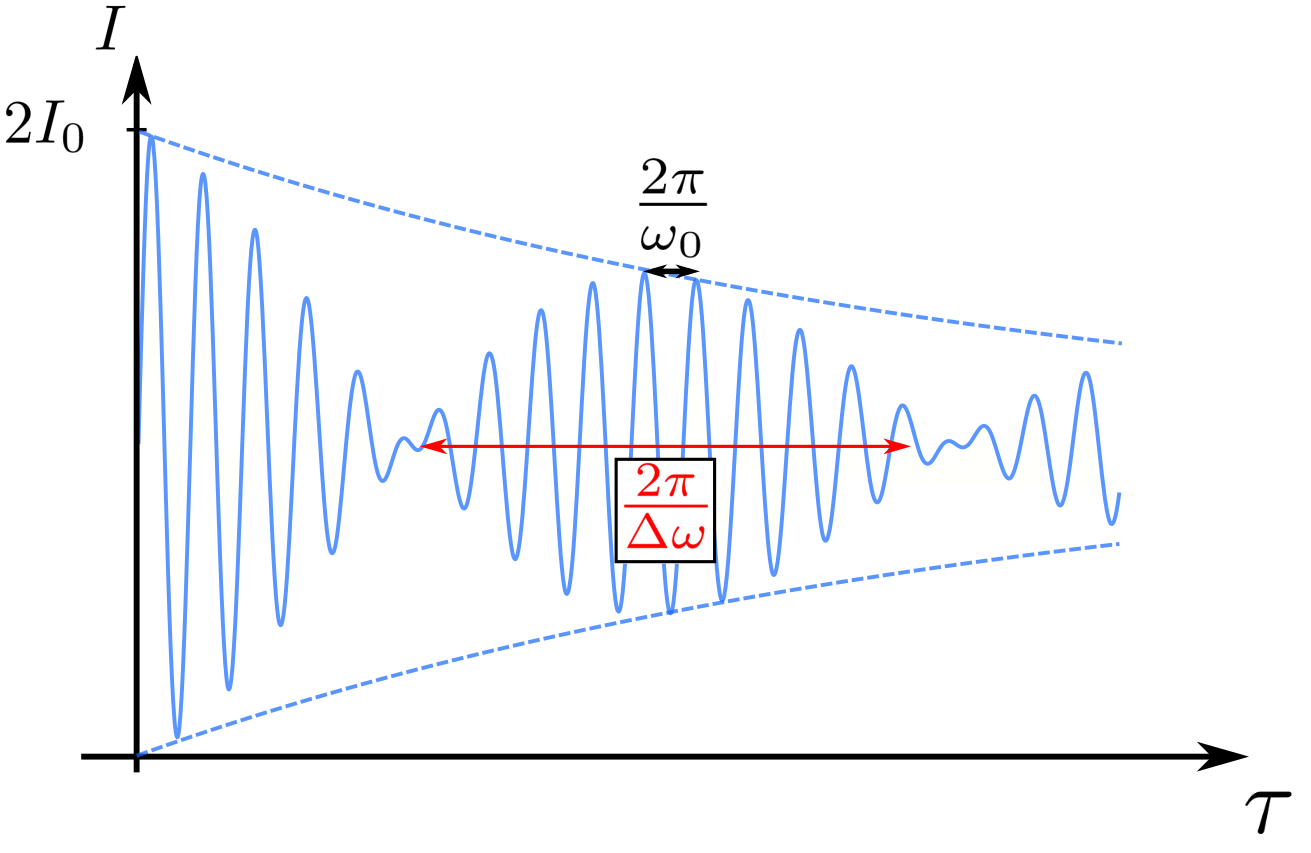
\includegraphics[width=0.78\textwidth]{Fig/Chapter1/michelson_two_lambda.png}
    \caption[Intensity pattern for a light source with two monochromatic component of frequencies $\omega_1$ and $\omega_2$]{Intensity pattern for a light source with two monochromatic component of frequencies $\omega_1$ and $\omega_2$. The fast oscillation of frequency $\omega_0=(\omega_1+\omega_2)/2$ is modulated by a slow oscillation of frequency $\Delta \omega = |\omega_1 - \omega_2|$ and an exponential decay $e^{-t/\tau_c}$.}
    \label{fig:michelson_two_lambda}
\end{figure}

Through this very simple example, we understand that the observed interference pattern strongly depends on the spectrum of the source. For a source with an arbitrary spectrum $S(\omega)$, under the assumption that every spectral components are independent and do not interfere with one another, the overall intensity pattern results of the sum of the contribution of each spectral component:

\begin{equation}
    I=\int_{-\infty}^{\infty} 2 S(\omega)[1+\cos (\omega \tau)] \mathrm{d} \omega
\end{equation}

\noindent Writing $\int_{-\infty}^{\infty} S(\omega) \mathrm{d} \omega=I_{0}$ and $s(\omega)=S(\omega) / I_{0}$, we obtain

\begin{equation}
    I=2 I_{0}\left[1+\int_{-\infty}^{\infty} s(\omega) \cos (\omega \tau) \mathrm{d} \omega\right]
\end{equation}

\noindent As $S(\omega) = |\mathrm{FT}[E(t)]|^2$ where FT denotes the Fourier transform, $s(\omega)$ is real allowing us to write \cite{mandel1995optical}:

\begin{equation}
    I=2 I_{0}\left[1+\mathrm{Re} \left(\int_{-\infty}^{\infty} s(\omega) \cos (\omega \tau) \mathrm{d} \omega\right)\right]
\end{equation}

\noindent From which we get, using equation \ref{eq:def_g1}:

\begin{equation}
    g^{(1)}(\tau)=\int_{-\infty}^{\infty} s(\omega) \mathrm{e}^{\mathrm{i} \omega \tau} \mathrm{d} \omega
\end{equation}

\noindent where we recognize the definition of the Fourier transform. This is the \textbf{Wiener-Khintchine} theorem. The first-order correlation function, measurable with an interferometric measurement, thus contains information about the spectrum of the light source. 



% Note that this is only one example in the ensemble of the many possible applications of the study of first-order correlation. We can also quote for instance the characterization of the spatial coherence of a non punctual source with the famous Young's slits experiment. 

In this introductory paragraph, we have seen a concrete and evocative example of how correlation functions can be used to obtain meaningful information about a given system, here a light source, with the simplest correlation function there is, correlating two values of the light field. This idea can be extended to higher order of correlations like intensity correlations, involving four values of the light field. This was at the core of the approach developed by Hanbury Brown and Twiss to improve the resolution of the Michelson interferometer to measure the size of the stars and avoid the deterrent effect of turbulences from the atmosphere in their celebrated 1954 article \cite{brown1954lxxiv}. This experiment was of particular importance as its interpretation in terms of individual particles, the photons, gave birth to the field of Quantum Optics. 





% At this point, the link with our initial goal, {\it i.e.} characterizing quantum many-body interacting systems, does not seem so clear. As we mentioned earlier, interactions induce correlations between several particles for which we will need higher order correlation functions. Let us now take the next step in this direction and look at \textbf{second-order correlation functions}. For the moment, we will keep things simple and work in the context of Optics, and thus with non-interacting particles, for which this formalism was historically developed and that provides well-known, easy to understand examples.

% The same reasoning can be conducted for the spatial coherence for instance with the non less famous Young double slit experiment. 

% We will not detail here all the intricacies of the study of first-order correlation functions for different light sources. The main point to remember is that the first order correlation function is a natural way to characterize the coherence properties of a light source and thus contains a lot of meaningful information.


\subsection{Second order correlation function of light: Hanbury Brown and Twiss experiment}

\begin{figure}
    \centering
    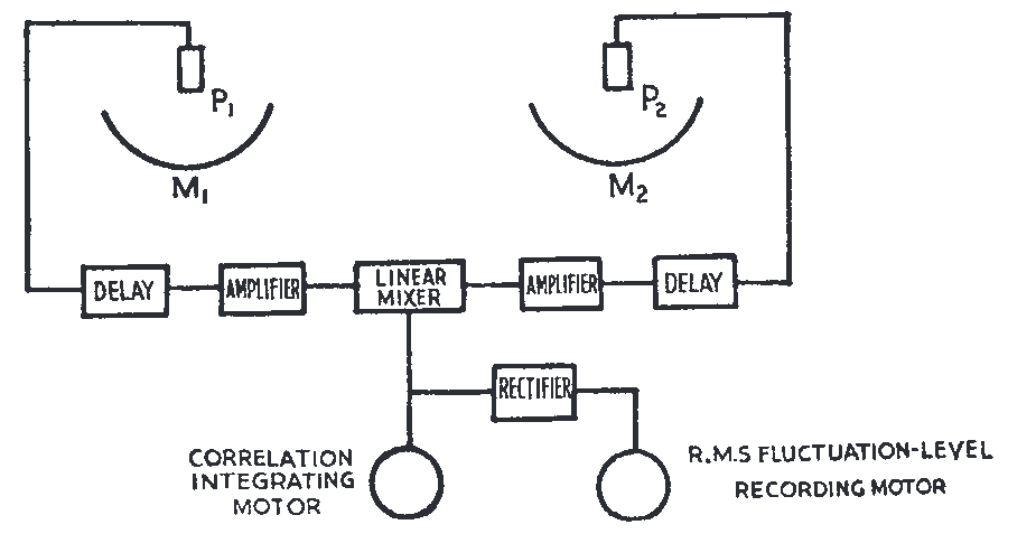
\includegraphics[width=0.7\textwidth]{Fig/Chapter1/HBT_apparatus.png}
    \caption[Diagram of the historical Hanbury Brown and Twiss apparatus]{Diagram of the historical Hanbury Brown and Twiss apparatus, taken from \cite{brown1956test}. The novelty of this apparatus was to use two detectors, $P_1$ and $P_2$, to measure the second-order correlation function.}
    \label{fig:HBT_apparatus}
\end{figure}

\label{sec:hbt_classical}

The scheme proposed by Hanbury Brown and Twiss relies on the measurement of cross-correlations between the intensities measured by two independent photodetectors (see Fig-\ref{fig:HBT_apparatus}), \ie a measurement of the \textbf{second-order correlation function}. To understand how it works, we will follow the complementary approach to the one developed in the last paragraph and look at the spatial properties of the light source. 

A star is described as an incoherent, extended light source that we approximate to be monochromatic (wavelength $\lambda$) for simplicity (in practice, filters can be used to obtain a quasi-monochromatic source). We write $S$ the surface of the source seen from the Earth. We model this source of light as an ensemble of elementary, point-like and independent emitters and note their spatial location $\bm{s}$. The field amplitude at a point $\bm{r}$ in an observation plane situated at distance $L$, far-away from the source so that we are in the Fraunhofer regime $L \gg \lambda, r,s$, writes (see Fig-.\ref{fig:source_and_plane}):

\begin{equation}
    E(\bm{r}) \propto \int_{S} e(\bm{s}) e^{\frac{i \pi}{\lambda L}|\bm{r}-\bm{s}|^{2}} d \bm{s}
    \label{eq:amp_HBT}
\end{equation}

\begin{figure}
    \centering
    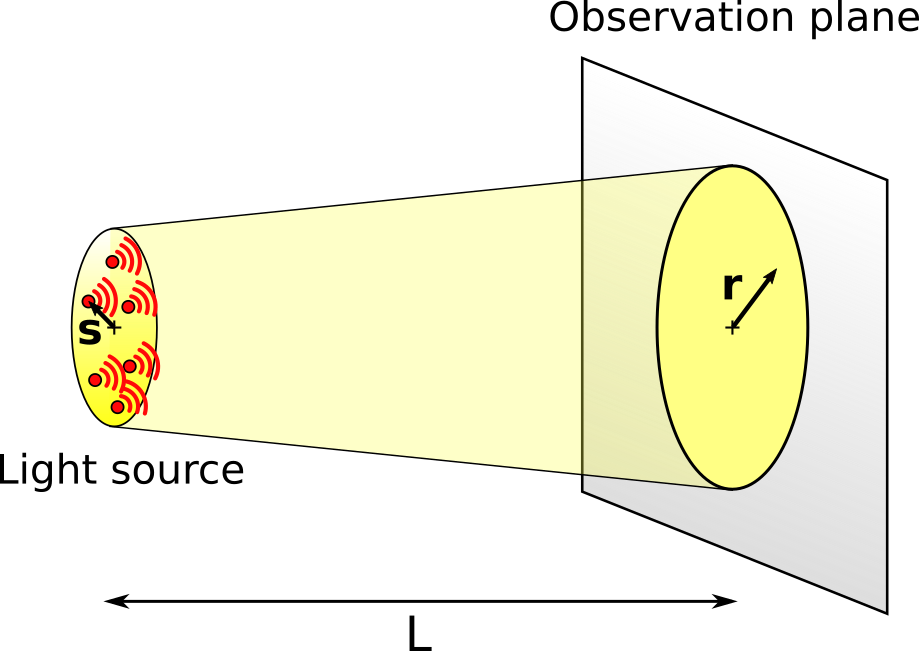
\includegraphics[width=0.7\textwidth]{Fig/Chapter1/source_and_plane.png}
    \caption[Schematic of an extended light source]{Schematic of an extended light source. The small red dots represent the different incoherent elementary emitters of the source.}
    \label{fig:source_and_plane}
\end{figure}

The second-order correlation function correlates the values of the intensity of the light field at two different points of space $\bm{r}_1$ and $\bm{r}_2$. In terms of field amplitude, it corresponds to the four-term correlator:

\begin{equation}
    G^{(2)} (\bm{r}_1,\bm{r}_2) = \mean{E^*(\bm{r}_1) E(\bm{r}_1) E^*(\bm{r}_2) E(\bm{r}_2)}
\end{equation}

\noindent All the elementary emitters are incoherent and thus each have a random phase value, determined by an uniform probability law defined on the interval $[0,2\pi[$. They thus form a set of \textbf{independent} random variables with the \textbf{same statistics}. We can therefore apply the Central Limit Theorem to the sum of their contributions $E(\bm{r})$ and find that it follows Gaussian statistics \cite{goodman2007speckle}. The fact that $E$ is a classical Gaussian variable allows us to simplify the four-term correlator into:

\begin{equation}
     G^{(2)} (\bm{r}_1,\bm{r}_2) = \mean{I(\bm{r}_1)} \mean{I(\bm{r}_2)} + \mean{E^*(\bm{r}_1) E(\bm{r}_2)} \mean{E(\bm{r}_1) E^*(\bm{r}_2)}
\end{equation}

\noindent We recognize in the second term the spatial counterpart of the temporal first-order correlation function discussed in the previous paragraph. Using equation \ref{eq:amp_HBT}, we obtain:

\begin{equation}
    G^{(1)}\left(\bm{r}_{1}, \bm{r}_{2}\right)=\left\langle E^*(\bm{r}_1) E(\bm{r}_2)\right\rangle \propto \iint_{S}\left\langle e^{*}(\bm{s}_1) e(\bm{s}_2)\right\rangle e^{-\frac{i \pi}{\lambda L}\left(\left|\bm{r}_{1}-\bm{s}_1\right|^{2}-\left|\bm{r}_{2}-\bm{s}_2\right|^{2}\right)} \mathrm{d} \bm{s}_1 \mathrm{d} \bm{s}_2
\end{equation}

\noindent Since the source is incoherent, $\left\langle e^{*}(\bm{s}_1) e(\bm{s}_2)\right\rangle = I(\bm{s}_1) \delta_{\bm{s}_1,\bm{s}_2}$, leading to

\begin{equation}
    G^{(1)}\left(\bm{r}_{1}, \bm{r}_{2}\right) \propto \iint_{S} I(\bm{s}_1) e^{-\frac{2 i \pi}{\lambda L}\left(\bm{r}_{1}-\bm{r}_{2}\right) \bm{s}_1} \mathrm{d} \bm{s}_1 d \bm{s}_2
\end{equation}

\noindent In analogy with what we showed in the last paragraph for the temporal coherence, the first-order spatial correlation function is the Fourier transform of the spatial intensity profile. This is known as the \textbf{Van Cittert-Zernike} theorem \cite{goodman2007speckle}. For a homogeneous intensity distribution of the source, the first-order correlation function decays on a length scale called the \textbf{correlation length} $l_c$ proportional to the inverse of the source size $L_{\mathrm{source}}$, $l_c \sim \lambda L / L_{\mathrm{source}}$.

In a nutshell, the second-order normalized correlation function takes the simple expression:

\begin{equation}
    \gtwo (\bm{r}_1,\bm{r}_2) = \frac{\mean{I(\bm{r}_1)} \mean{I(\bm{r}_2)} + \mean{E^*(\bm{r}_1) E(\bm{r}_2)} \mean{E(\bm{r}_1) E^*(\bm{r}_2)}}{\mean{I(\bm{r}_1)}\mean{I(\bm{r}_2)}} = 1 + |g^{(1)}(\bm{r}_1,\bm{r}_2)|^2
\end{equation}

\noindent Depending on the positions of the detectors $\bm{r}_1$ and $\bm{r}_2$ we have (see Fig.-\ref{fig:g2_HBT_illu}:

\begin{itemize}
    \item $\gtwo (\bm{r}_1,\bm{r}_2)=2$ for $\bm{r}_1=\bm{r}_2$
    \item $1 \leq \gtwo (\bm{r}_1,\bm{r}_2) \leq 2$ for $|\bm{r}_1-\bm{r}_2| \lesssim l_{c}$
    \item $\gtwo (\bm{r}_1,\bm{r}_2)=1$ for $|\bm{r}_1-\bm{r}_2| \gg l_{c}$
\end{itemize}

\begin{figure}
    \centering
    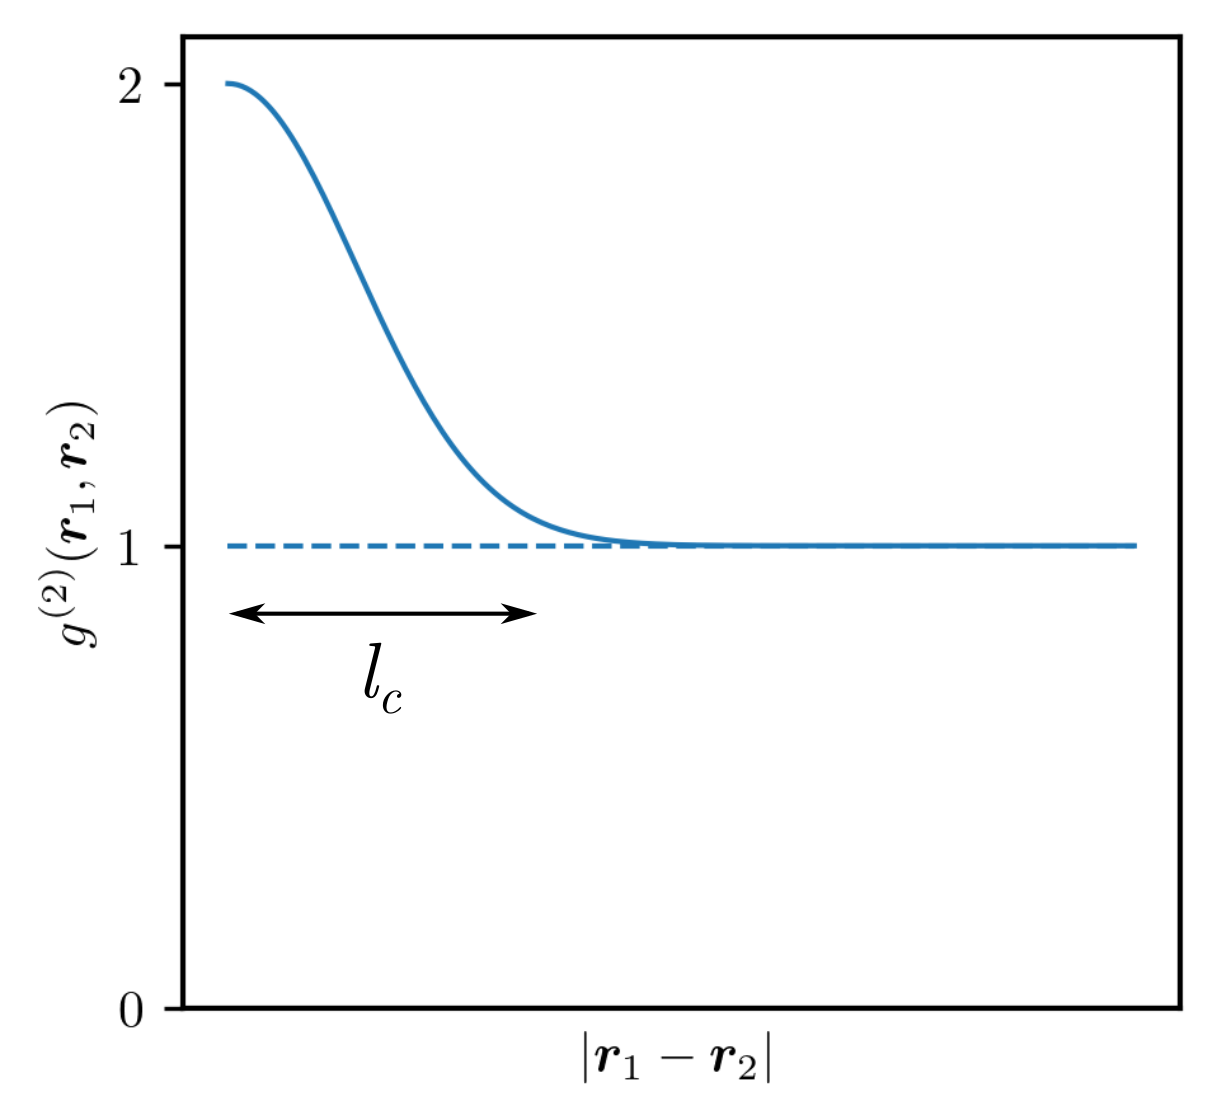
\includegraphics[width=0.6\textwidth]{Fig/Chapter1/g2_HBT_illu.png}
    \caption[Second-order normalized correlation function for the Hanbury Brown and Twiss effect]{Second-order normalized correlation function for the Hanbury Brown and Twiss effect.}
    \label{fig:g2_HBT_illu}
\end{figure}

\noindent The size of the source can thus be measured by progressively increasing the distance between the two detectors and measuring the length scale on which the second order correlation function decreases. This was done successfully by Hanbury Brown and Twiss \cite{brown1956test} to measure the size of Sirius in 1956.

While the calculations are rather straightforward in a classical model where light is described as a wave, the interpretation of the Hanbury Brown and Twiss experiment in terms of individual particles, \ie from a Quantum Optics point of view, sparked many debates that lead to a deeper understanding of the phenomena involved. If we take a look at what happens for $\bm{r}_1=\bm{r}_2$, we see that a peculiar phenomenon occurs. The normalized second-order correlation function can be interpreted as the probability to detect simultaneously two photons on the detector located at $\bm{r}_1$ and $\bm{r}_2$, normalized by the probability to detect them independently. Therefore, since $\gtwo (\bm{r}_1,\bm{r}_2)=2$ for $\bm{r}_1=\bm{r}_2$, the probability to detect two photons at the same position is twice as high as it is to detect them independently! It was only after a few years that an explanation was suggested by Fano in 1961 \cite{fano1961quantum}. Considering a pair of source points A and B in the star and two detectors 1 and 2 on Earth, Fig-.\ref{fig:HBT_scheme} illustrates the two possibilities for a joint detection of two photons on the couple of detectors. For indistinguishable photons, the paths amplitudes interfere constructively resulting in a joint detection probability higher than that for independent events. While the interference effect is averaged out considering all the possible pairs of elementary emitters in the source, it can be observed when the distance between the two detectors is very close to zero, as observed by Hanbury Brown and Twiss. Interestingly, the interferences are destructive for fermions, resulting in a reduced probability of joint detection, also referred as \textbf{anti-bunching}, an effect than cannot be explained classically contrary to the Hanbury Brown and Twiss effect. 

\begin{figure}
    \centering
    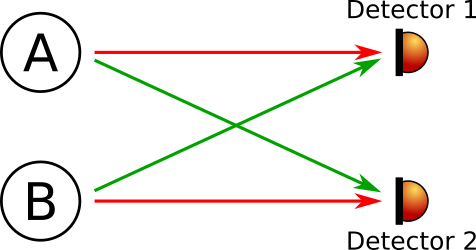
\includegraphics[width=0.55\textwidth]{Fig/Chapter1/HBT_scheme.png}
    \caption[Quantum interpretation of the Hanbury Brown and Twiss effect]{Quantum interpretation of the Hanbury Brown and Twiss effect. For two source points A and B, a joint detection occurs if a photon produced by A is detected in 1 and a photon produced by B is detected in 2 (red arrows), or the other way around A $\rightarrow$ 2 and B $\rightarrow$ 1 (green arrows). Interferences of the paths amplitudes explain the Hanbury Brown and Twiss effect.}
    \label{fig:HBT_scheme}
\end{figure}

Because it will be a crucial point in the following of this thesis, we stress that the key ingredient to observe bosonic bunching is the \textbf{chaotic} character of the source. The theoretical development that we have just presented relies on the application of the Central Limit Theorem for the source made of a large number of independent elementary emitters, each with a random phase. This is notably not the case for laser light that we will discuss in the next paragraph.

% This is notably not the case for laser light which is fully coherent and results in $\gtwo (\bm{r}_1,\bm{r}_2)=1$ for all values of $\bm{r}_1$ and $\bm{r}_2$.

To summarize, we have seen in this paragraph an example of a second-order correlation effect, the Hanbury Brown and Twiss effect, and its classical description with a chaotic light source. We also have an insight of how this effect can be understood when considering individual particles, here photons, laying the grounds to study more complex systems with correlations between interacting quantum particles. The observations of Hanbury Brown and Twiss sparked interest in the community and lead to the development of the new formalism of Quantum Optics \cite{glauber1963quantum} with quantized light fields or light particles, {\it i.e.} photons, with the great success that we know of today. In the next paragraphs, we will study the main elements of the theory of Quantum Optics through a few examples of increasing complexity as a mean to understand and conceptualize correlations at the single particle level.

\subsection{Second quantization and correlations between individual particles}

The first quantum descriptions, such as the one developed by Planck to describe black-body radiation, were in fact semi-classical theories in the sense that only the energy of the atoms is quantized, while the radiation fields are still described classically. While semi-classical theories found great success, the observations of Hanbury Brown and Twiss, as well as the development of laser light called for a theory accounting for the corpuscular aspect of light. This gave birth to the Quantum Optics theory whose core element is to push further the idea of quantization by quantizing the radiation fields. While the term is most often associated with atomic physics as we will see later on, we can speak here of \textbf{second quantization}, the first quantization being the one of the energy.

The general idea behind the quantization of the light field is to describe light as a collection of independent quantum harmonic oscillators for the different modes of the field. For a field defined in a box of volume $V=L^3$ with periodic boundary conditions, the field can be described as a superposition of plane waves with a wave vector $k=\frac{2 \pi}{L} n$ with $n \in \N$ each described by a harmonic oscillator \cite{walls2008}:

\begin{equation}
    \hat{\bm{E}}(\bm{r}, t)=\sum_{l} i \bm{\epsilon}_{l} \sqrt{\frac{\hbar \omega_l}{2 \varepsilon_0 V}} \left[e^{i (\bm{k}_{l} \cdot \bm{r} - \omega_l t)} \hat{a}_{l}-e^{-i (\bm{k}_{l} \cdot \bm{r} - \omega_l t)} \hat{a}_{l}^{\dagger}\right]  = \hat{\bm{E}}^{(+)}(\bm{r}, t)+\hat{\bm{E}}^{(-)}(\bm{r}, t)
\end{equation}

\noindent where $\bm{\epsilon}_{l}$ denotes the polarisation of mode $l$. We have introduced the two mutually adjoint operators $\hat{a}_{l}$ and $\hat{a}_{l}^{\dagger}$, analog to the creation and annihilation operators of the quantum harmonic oscillator. In the formalism of the quantum harmonic oscillator, these operators respectively destroy or create a quanta of energy, which in our case corresponds to a photon in mode $l$. Since photons are bosons, $\hat{a}_{l}$ and $\hat{a}_{l}^{\dagger}$ follow the commutation relations:

\begin{equation}
    \left[\hat{a}_{l}, \hat{a}_{l^{\prime}}^{\dagger}\right]=\delta_{l l^{\prime}} \quad\left[\hat{a}_{l^{\prime}}, \hat{a}_{l}\right]=0
\end{equation}

To show the effect of $\hat{a}_{l}$ and $\hat{a}_{l}^{\dagger}$, we introduce the \textbf{number states} or \textbf{Fock states} $\ket{n_l}$, eigenstates of the number operator $\hat{N}_l = \hat{a}_{l}^{\dagger} \hat{a}_{l}$ with $n_l$ representing the number of photons in mode $l$. The Fock state corresponding to the absence of the photons is called the vacuum state and denoted $\ket{0}$. The action of the creation and annihilation operators on the Fock states writes:



\begin{equation}
    \hat{a}_{l}^{\dagger} \ket{n_l}=\sqrt{n_l+1}\left|n_l+1\right\rangle
\end{equation}
\begin{equation}
    \hat{a}_{l} \ket{n_l}=\sqrt{n_l}\left|n_l-1\right\rangle
\end{equation}

\noindent From this, we see that every Fock state can be obtained by applying the creation operator on the vacuum state the right amount of times:

\begin{equation}
    \left|n_{l}\right\rangle=\frac{1}{\sqrt{n_{l} !}}\left(\hat{a}_{l}^{\dagger}\right)^{n_{l}}\left|0\right\rangle
\end{equation}


\noindent Finally we can write the Hamiltonian of the collection of independent quantum harmonic oscillators as:

\begin{equation}
    \hat{H}=\sum_{l} \hbar \omega_{l}\left(\hat{N}_{l}+\frac{1}{2}\right)
\end{equation}

\noindent with $\hbar \omega_l$ being the energy of a photon in mode $l$.

\subsubsection{n-th order correlation functions}

As discussed in the previous paragraphs, there is a strong connection between correlation functions and the notion of coherence. Motivated by the measurements of Hanbury Brown and Twiss, Roy J. Glauber introduced \cite{glauber1963quantum} the notion of $n$-th order coherence in the formalism of Quantum Optics and linked it to $n$-th order correlation functions, as we will recall now.

We have discussed so far correlation functions up to the second order. Correlation functions can be extended to higher order $n$ describing the probability of joint detection of $n$ photons at a set of positions and times $\{(\bm{r}_1,t_1),(\bm{r}_2,t_2),...,(\bm{r}_n,t_n)\}$: 

\begin{equation}
    G^{(n)}\left(\bm{r}_{1}, t_{1}, ... , \bm{r}_{n}, t_{n}\right)=\left\langle \hat{\bm{E}}^{(-)}\left(\bm{r}_{1}, t_{1}\right) ... \hat{\bm{E}}^{(-)}\left(\bm{r}_{n}, t_{n}\right) \hat{\bm{E}}^{(+)}\left(\bm{r}_{n}, t_{n}\right) ... \hat{\bm{E}}^{(+)}\left(\bm{r}_{1}, t_{1}\right)\right\rangle
\end{equation}

\label{sec:normal_order}
\noindent Note that the order of the operators is important with all the terms in $\hat{E}^{(-)}$ (and thus $\hat{a}^{\dagger}$) on the left and terms in $\hat{E}^{(+)}$ (and thus $\hat{a}$) on the right. This is called \textbf{normal ordering} and ensures that the expectation value of the combination of the operators is zero for the vacuum state. 

Likewise, we introduce the normalized $n-$th order correlation function.

\begin{equation}
    g^{(n)}\left(\bm{r}_{1}, t_{1}, ...,  \bm{r}_{n}, t_{n}\right)=\frac{G^{(n)}\left(\bm{r}_{1}, t_{1}, ...,  \bm{r}_{n}, t_{n}\right)}{\displaystyle \prod_{j=1}^{n} G^{(1)}\left(\bm{r}_{1}, t_{1}, ..., \bm{r}_{n}, t_{n}\right)}
\end{equation}

\subsubsection{Coherent states}

\noindent From this definition, we define a fully coherent field as a field that verifies, for any value of $n \in \N^*$ \cite{glauber1963quantum}:

\begin{equation}
    g^{(n)}\left(\bm{r}_{1}, t_{1}, ...,  \bm{r}_{n}, t_{n}\right)  = 1
    \label{eq:cond_g_coherent}
\end{equation}

\noindent This means that for a fully coherent field, we have the simple relation:

\begin{equation}
    G^{(j)}\left(\bm{r}_{1}, t_{1}, ... , \bm{r}_{j}, t_{j}\right) = \prod_{i=1}^{j} G^{(j)}(\bm{r}_{i}, t_{i})
    \label{eq:cond_G_coherent}
\end{equation}

Interestingly, we note that if the field was in a state $\ket{\alpha}$ that would be an eigenstate of $\hat{\bm{E}}^{(+)}$, $\hat{\bm{E}}^{(+)} \ket{\alpha} = \alpha \ket{\alpha}$, and an eigenstate of $\hat{\bm{E}}^{(-)}$, $\bra{\alpha} \hat{\bm{E}}^{(-)} = \bra{\alpha} \alpha^*$, the conditions \ref{eq:cond_g_coherent} and \ref{eq:cond_G_coherent} would be automatically verified. For simplicity sake, we consider a single mode and use the fact that $\hat{\bm{E}}^{(+)} \propto \hat{a}$ and $\hat{\bm{E}}^{(-)} \propto \hat{a}^{\dagger}$. We are thus looking for the state $\ket{\alpha}$ which is an eigenstate of $\hat{a}$. It can be shown that in the basis of the number states, $\ket{\alpha}$ writes \cite{glauber1963coherent}:

\begin{equation}
    |\alpha\rangle=e^{-\frac{1}{2}|\alpha|^{2}} \sum_{n=0}^{\infty} \frac{\alpha^{n}}{\sqrt{n !}}|n\rangle
    \label{eq:coherent_state}
\end{equation}

\noindent The state $\ket{\alpha}$ is called a \textbf{coherent state} or Glauber state. We thus find that a coherent state writes as a sum of number states and that the probability to find $n$ photons follows a Poissonian law (see Fig.-\ref{fig:light_statistics}). A well-known example of coherent state is laser light.

Let us now close the parenthesis on the coherent state and come back to the Hanbury Brown and Twiss effect described in the last sub-section, characterized by $\gtwo (\bm{r}_1, t_1, \bm{r}_2, t_2) = 2$ for $\bm{r}_1 = \bm{r}_2$ and $t_1=t_2$. As we have just seen, it would be impossible to observe this effect with a fully coherent light as $\gtwo (\bm{r}_1, t_1, \bm{r}_2, t_2) = 1$ by definition. Let us rewrite the second order correlation function in the formalism of Quantum Optics to see if it tells us something new. For $\bm{r}_1 = \bm{r}_2$ and $t_1=t_2$, the expression writes: 

\begin{equation}
     g^{(2)}\left(\bm{r}_{1}, t_{1}, \bm{r}_{2}=\bm{r}_1, t_{2}=t_1\right) = \frac{\left\langle\hat{a}^{\dagger} \hat{a}^{\dagger} \hat{a} \hat{a}\right\rangle} {\left\langle\hat{a}^{\dagger} \hat{a}\right\rangle^{2}}
\end{equation}

\noindent Using the commutation relation, we write:

\begin{equation}
    g^{(2)}\left(\bm{r}_{1}, t_{1}, \bm{r}_{2}=\bm{r}_1, t_{2}=t_1\right) = \frac{\left\langle\hat{a}^{\dagger} ( \hat{a} \hat{a}^{\dagger}-1) \hat{a} \right\rangle} {\left\langle\hat{a}^{\dagger} \hat{a}\right\rangle^{2}} = \frac{\mean{N^2}-\mean{N}}{\left\langle\hat{a}^{\dagger} \hat{a}\right\rangle^{2}}  = 1 +  \frac{\sigma^2_N-\mean{N}}{\left\langle\hat{a}^{\dagger} \hat{a}\right\rangle^{2}}
    \label{eq:g2_variance}
\end{equation}

\noindent where we introduce $\sigma_N$ the standard deviation of the number of photons N. We see that the value of $\gtwo$ depends on the statistics of the source. For the case of laser light where $N$ follows a Poissonian law, $\sigma_N^2 = \mean{N}$ and we retrieve $g^{(2)}\left(\bm{r}_{1}, t_{1}, \bm{r}_{2}=\bm{r}_1, t_{2}=t_1\right) = 1$.

\subsubsection{Thermal chaotic states}

To understand how the Hanbury Brown and Twiss effect arises, we need to introduce the concept of \textbf{mixed states}, in opposition to \textbf{pure states}. In most cases, our limited knowledge of the system requires to describe it as a statistical mixture of pure states. This is what we call a mixed state. For such states, we use the formalism of the \textbf{density matrix} which is defined as:

\begin{equation}
    \hat{\rho} = \sum_{i} p_i \ket{\Psi_i} \bra{\Psi_i}
\end{equation}

\noindent where $p_i$ is the probability for the system to be in the pure state $\ket{\Psi_i}$. The expectation value of an operator $\hat{O}$ is obtained through:

\begin{equation}
    \mean{\hat{O}} = \rm{Tr}(\hat{\rho} \hat{O})
\end{equation}

\begin{figure}
    \centering
    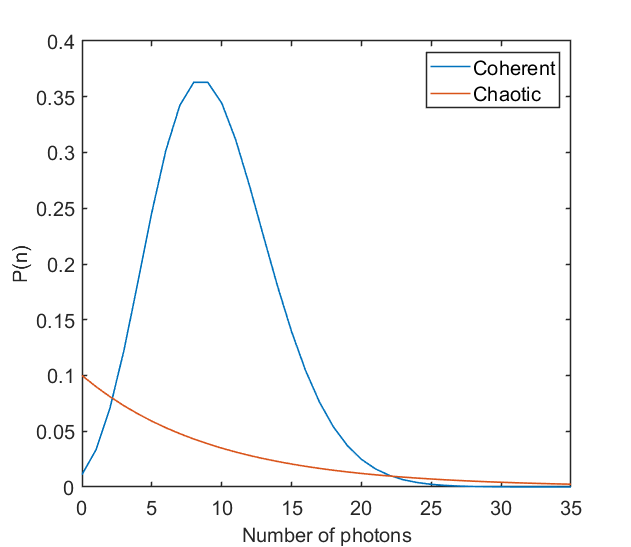
\includegraphics[width=0.63\textwidth]{Fig/Chapter1/coherent_vs_chaotic.png}
    \caption[Probability distribution of photon numbers for coherent and chaotic light sources]{Probability distribution of the number of photons for coherent and chaotic light sources for a fixed value of $|\alpha^2|$.}
    \label{fig:light_statistics}
\end{figure}

This formalism is particularly useful to describe light sources made of a large number of independent individual emitters. Let us say that the first emitter brings the field in state $\ket{\alpha_1}$, the second emitter in state $\ket{\alpha_2}$ etc.. It can be shown (\cite{glauber1963coherent}) that for a large number of individual emitters $j$, the probability distribution for the complex amplitude $\alpha=\alpha_1 + \alpha_2 + ... + \alpha_j$ follows a Gaussian law:

\begin{equation}
    P(\alpha)= \frac{1}{\pi \mean{n}} e^{-\frac{|\alpha|^2}{\mean{n}}}
    \label{eq:p_alpha}
\end{equation}

\noindent where $\mean{n}$ is the mean value of $|\alpha|^2$ and represents the number of energy quanta in the mode. From this, we use equation \ref{eq:coherent_state} to write the density matrix of the system in the basis of the number states:

\begin{equation}
    \hat{\rho}=\frac{1}{1+\langle n\rangle} \sum_{m=0}^{\infty}\left(\frac{\langle n\rangle}{1+\langle n\rangle}\right)^{m}|m\rangle\langle m|
    \label{eq:rho_chaotic}
\end{equation}

\noindent The probability to find $m$ photons then writes (see Fig.-\ref{fig:light_statistics}):

\begin{equation}
    P(m)=\frac{1}{1+\langle n\rangle}\left(\frac{\langle n\rangle}{1+\langle n\rangle}\right)^{m}
    \label{eq:chaotic_light}
\end{equation}


\noindent A light source with these statistics is called a \textbf{chaotic} light source. This is notably the case of thermal light, described by the Planck's distribution with $\mean{n}=1/(e^{h\nu/\kB T}-1)$. From equation \ref{eq:chaotic_light}, we find that the variance of the photon number $N$ writes:

\begin{equation}
    \sigma_N^2=\mean{N}^2+\mean{N}
\end{equation}

\noindent Injecting this result into equation \ref{eq:g2_variance}, we find that for a chaotic light source, \\ $g^{(2)}\left(\bm{r}_{1}, t_{1}, \bm{r}_{2}, t_{2}\right)=2$ for $\bm{r}_{1}=\bm{r}_{2}$ and $t_1=t_2$, that is the bosonic bunching observed by Hanbury Brown and Twiss!



% For chaotic thermal light, the photons statistics are set by the Bose-Einstein statistics giving $\sigma_N^2=\mean{N}^2+\mean{N}$, we find back $g^{(2)}=2$! On the other hand, for the coherent light of a laser, the standard deviation of the photon number is set by the shot noise $\sigma_N^2=N$ and we retrieve $g^{(2)}=1$.

In fact, this result can be obtained through a complementary approach that relies on the application of the Wick's theorem \cite{gardiner2004quantum}.

\subsubsection{Wick's theorem}

\begin{tcolorbox}[colback=red!5!white,colframe=red!75!black,title=\textbf{Wick's theorem}]
\label{sec:wick}
When a system is characterized by a Gaussian density matrix \cite{gardiner2004quantum} \\ $\hat{\rho} \propto \exp(\sum_i ( \alpha_i \hat{a}_i^{\dagger} \hat{a}_i^2 + \beta_i \hat{a}_i^2 + \gamma_i \hat{a}_i^{\dagger}^2))$ and $\forall i, \langle \hat{a}_i} \rangle =\langle \hat{a}^{\dagger}_i \rangle=0$, the high-order products of of creation and annihilation operators can be factorized into all possible products of only two operators. For bosonic particles, this writes:

$$ \mean{\hat{A}_1 ... \hat{A}_{2m}} = \sum_{\sigma} \mean{\hat{A}_{i_1} \hat{A}_{i_2}} \mean{\hat{A}_{i_3} \hat{A}_{i_4}} ... \mean{\hat{A}_{i_{2m-1}} \hat{A}_{i_{2m}}}$$

where $\sigma$ denotes all possible permutations changing the order $1,2,...,2m$ to $i_1,i_2,...,i_{2m}$, and $\hat{A}_i$ is any creation or annihilation operator.

\end{tcolorbox}

As shown in equations \ref{eq:p_alpha} and \ref{eq:rho_chaotic}, the density matrix of a chaotic light source is Gaussian, it is therefore possible to use Wick's theorem to simplify the second-order correlation function 

%exactly as we did classically in \ref{sec:hbt_classical} :

\begin{equation}
     g^{(2)}\left(\bm{r}_{1}, t_{1}, \bm{r}_{2}=\bm{r}_1, t_{2}=t_1\right) =\frac{ \langle \hat{a}^{\dagger} \hat{a}^{\dagger} \rangle \mean{\hat{a} \hat{a}} + 2\langle \hat{a}^{\dagger} \hat{a} \rangle^2}{\langle \hat{a}^{\dagger} \hat{a} \rangle ^2}
     \label{eq:g2_wick}
\end{equation}

\noindent For a thermal chaotic state where the number of photons is well defined, the averages $\langle \hat{a}^{\dagger} \hat{a}^{\dagger} \rangle$ and $\mean{\hat{a} \hat{a}}$ are null as they do not conserve the number of photons. We thus retrieve that $g^{(2)}\left(\bm{r}_{1}, t_{1}, \bm{r}_{2}=\bm{r}_1, t_{2}=t_1\right)=2$. Actually, this procedure can be extended up to any order to show that the $n$-th order correlation function can be simplified to a linear combination of first-order correlation functions. This means that the entirety of the information is contained in the first-order correlation function. The normalized probability of joint detection of $n$ photons then writes:

\begin{equation}
    g^{(n)} (\bm{r}_1,...,\bm{r}_n,t_1,...,t_n) = n! \ \mathrm{for} \ \bm{r}_1=\bm{r}_2= ... =\bm{r}_n \ \mathrm{and} \ t_1=t_2=...=t_n
\end{equation}

\noindent which is a generalisation of the two particles bosonic bunching, seen previously, for $n$ particles. Importantly, the situation is very different with a coherent state $\ket{\alpha}$ as we have $\langle \hat{a} \rangle, \langle \hat{a}^{\dagger} \rangle, \mean{\hat{a} \hat{a}}, \langle \hat{a}^{\dagger} \hat{a}^{\dagger} \rangle \neq 0$ (because the well defined phase implies that the photon number is not defined). While the Wick's theorem still applies, its expression is more complicated and not helpful as the second order correlation function is much easier to compute:


\begin{equation}
     g^{(2)}\left(\bm{r}_{1}, t_{1}, \bm{r}_{2}=\bm{r}_1, t_{2}=t_1\right) = \frac{\bra{\alpha} \hat{a}^{\dagger} \hat{a}^{\dagger} \hat{a} \hat{a} \ket{\alpha}} {\bra{\alpha} \hat{a}^{\dagger} \hat{a} \ket{\alpha}^{2}} = \frac{|\alpha|^4}{|\alpha|^4}=1
\end{equation}

\label{sec:coherent_g2}

\noindent This proves that coherent states do not show bosonic bunching.

We have thus seen how the Hanbury Brown and Twiss effect writes in the formalism of Quantum Optics and shown the differences between a coherent and chaotic light source. We will keep this result in the back of our minds as it will be of primary importance when we will study second order correlation functions with interacting atoms a little further down the line.

\subsection{The non-degenerate parametric amplifier}

\label{sec:amp_parametric}

We will now increase the complexity by adding non-linearity in the systems we study as a means to induce additional correlations between different modes. The most emblematic example of such a system in Quantum Optics is the \textbf{non-degenerate parametric amplifier}. Through the interaction with a non-linear optical medium, a pump photon at frequency $2 \omega$ can be converted into two photons in two modes at frequency $\omega_1$ and $\omega_2$, the signal and idler mode that we name mode 1 and mode 2, with $2 \omega = \omega_1 + \omega_2$. Using a few approximations (see \cite{walls2008}), the Hamiltonian of the system may be written as:

\begin{equation}
    H=\hbar \omega_1 \hat{a}_1^{\dagger} \hat{a}_1+ \hbar \omega_2 \hat{a}_2^{\dagger} \hat{a}_2 + i \hbar \chi (\hat{a}_1^{\dagger}  \hat{a}_2^{\dagger} e^{-2i\omega t} - \hat{a}_1 \hat{a}_2 e^{2i\omega t})
\end{equation}

\noindent where $\chi$ is a coupling constant. The particularity of the two photons produced from the pump photon is that they are emitted in a correlated manner as a \textbf{pair}. The system will thus feature \textbf{cross-correlations} between the modes $1$ and $2$. 

% The non-degenerate parametric amplifier was used in landmark experiments \cite{burnham1970,heidmann1987observation} to demonstrate important results of quantum mechanics that were later reproduced with pairs of atoms instead of pairs of photons \cite{bucker2011,dall2009paired,perrin2007observation}. Understanding the physics of this system is then of primary importance for the kinds of experiment we which to conduct \NOTE{bof}.

% We thus have a direct analogy with the weakly-interacting Bose gas, the modes 1 and 2 being the analogues of the momentum modes $\bm{k}$ and $-\bm{k}$. This comparison does not come out of the blue as this system was used in landmark experiments \cite{burnham1970,heidmann1987observation} to demonstrate important results of quantum mechanics that were later reproduced with pairs of atoms instead of pairs of photons \cite{bucker2011,dall2009paired,perrin2007observation}. As we will now see, these observations also applies for the \kmk pairs of the quantum depletion that we wish to study.

This time-dependent problem is best solved in the interaction picture, {\it i.e.} where the time dependence is carried by both operators and states. The interaction Hamiltonian then writes:

\begin{equation}
    \hat{H}_I(t)=i \hbar \chi (\hat{a}_1^{\dagger}(t)  \hat{a}_2^{\dagger}(t) - \hat{a}_1(t) \hat{a}_2(t))
\end{equation}

\noindent The counterpart to the Schrödinger equation in the interaction picture is the Heisenberg equation of motion:

\begin{equation}
    \frac{\mathrm{d}\hat{a}_1}{\mathrm{d}t}= \frac{1}{i\hbar} [\hat{a}_1,2hat{H}_I]=\chi \hat{a}_2^{\dagger}
\end{equation}
\begin{equation}
    \frac{\mathrm{d}\hat{a}_2^{\dagger}}{\mathrm{d}t}= \frac{1}{i\hbar} [\hat{a}_2^{\dagger},\hat{H}_I]=\chi \hat{a}_1
\end{equation}

\noindent The solution of these coupled equations are:

\begin{equation}
    \hat{a}_1(t)=\hat{a}_1(0) \mathrm{cosh} \chi t + \hat{a}_2^{\dagger}(0) \rm{sinh} \chi t
    \label{eq:a1}
\end{equation}
\begin{equation}
    \hat{a}_2(t)=\hat{a}_2(0) \mathrm{cosh} \chi t + \hat{a}_1^{\dagger}(0) \rm{sinh} \chi t
    \label{eq:a2}
\end{equation}

\noindent From this, we can derive a few interesting results. First, we write the quantum state $\ket{\Psi(t)}$ generated by the parametric amplification process. To do so, we write the interaction picture evolution operator:

\begin{equation}
    \hat{U}(t)=\exp \left[\chi t\left(\hat{a}_{1}^{\dagger} \hat{a}_{2}^{\dagger}+\hat{a}_{1} \hat{a}_{2}\right)\right]
\end{equation}

\noindent At the price of a few lines of calculations (see \cite{schumaker1985new}), this operator can be re-written in a factored form:

\begin{equation}
    \hat{U}(t)=\frac{1}{(\cosh \chi t)} e^{\hat{a}_{1}^{\dagger} \hat{a}_{2}^{\dagger} \tanh \chi t} e^{-\left(\hat{a}_{1}^{\dagger} \hat{a}_{1}+\hat{a}_{2}^{\dagger} \hat{a}_{2}+1\right) \ln (\cosh \chi t)} e^{-\hat{a}_{1} \hat{a}_{2} \tanh \chi t}
\end{equation}

\noindent While this expression is a bit daunting, it becomes way simpler if we consider the initial state to be the vacuum:

\begin{equation}
    \ket{\Psi(t)} = \frac{1}{(\cosh \chi t)} e^{\hat{a}_{1}^{\dagger} \hat{a}_{2}^{\dagger} \tanh \chi t} \ket{0}
\end{equation}

\noindent We obtain easily from this the expression of $\ket{\Psi(t)}$ in the number states basis:

\begin{equation}
    |\Psi(t)\rangle=\frac{1}{(\cosh \chi t)} \sum_{n=0}^{\infty}(\tanh \chi t)^{n} \ket{n}_1 \ket{n}_2
\end{equation}

\label{sec:correlated_pop}

\noindent The state thus writes as a superposition of number states with the same number of photons in modes 1 and 2. The populations in modes 1 and 2 are therefore \textbf{perfectly correlated}. If we now look at the reduced state corresponding to mode 1 for instance, the reduced density matrix writes:

\begin{equation}
    \hat{\rho}_1 (t) = \mathrm{Tr}_2 \left[ \ket{\Psi(t)} \bra{\Psi(t)} \right] = \frac{1}{\cosh^2 \chi t} \sum_{n=0}^{\infty}\tanh^{2n} \chi t \ket{n}_1 \bra{n}_1
\end{equation}

\noindent Using the properties of hyperbolic functions, we get:

\begin{equation}
 \hat{\rho}_1 (t) = \frac{1}{1+ \sinh^2 \chi t} \sum_{n=0}^{\infty} \left( \frac{\sinh^2 \chi t}{1+\sinh^2 \chi t} \right)^n \ket{n}_1 \bra{n}_1
\end{equation}

\noindent where we recognize the form of the chaotic density matrix defined in equation \ref{eq:rho_chaotic} with $\mean{n} = \sinh^2 \chi t$. This result tells us that if we look only at one of the two modes and ignore the paired photons in the other mode, we observe bosonic bunching \cite{yurke1987} \fcolorbox{red}{white}{$g^{(2)} (1,1) = g^{(2)} (2,2) = 2$}.


\subsubsection{Amplitude of cross-correlations}

We have seen that the pairing process induces the presence of cross-correlations between modes 1 and 2 that can once again be characterized with the second-order correlation function. To look for a signature of these correlations, we compute the two-body correlator $G^{(2)}(1,2) =\langle \hat{a}_1^{\dagger}(t) \hat{a}_2^{\dagger}(t) \hat{a}_2(t) \hat{a}_1(t) \rangle$ which describes the probability to detect simultaneously a photon in mode 1 and a photon in mode 2. As explained in the last paragraph, we apply Wick's theorem and use equations \ref{eq:a1} and \ref{eq:a2} to get:

\begin{equation}
\begin{split}
    \langle \hat{a}_1^{\dagger}(t) \hat{a}_2^{\dagger}(t) \hat{a}_1(t) \hat{a}_2(t) \rangle = \langle \hat{a}_1^{\dagger}(t) \hat{a}_2^{\dagger}(t) \rangle \langle \hat{a}_1(t) \hat{a}_2(t) \rangle +  \langle \hat{a}_1^{\dagger}(t) \hat{a}_1(t) \rangle \langle \hat{a}_2^{\dagger}(t) \hat{a}_2(t) \rangle \\
    +  \langle \hat{a}_1^{\dagger}(t) \hat{a}_2(t) \rangle \langle \hat{a}_2^{\dagger}(t) \hat{a}_1(t) \rangle
\end{split}
\label{eq:wick_NDPA}
\end{equation}

\noindent Working with initial vacuum conditions, we compute the different correlators:

\begin{equation}
\begin{split}
   \langle \hat{a}_1(t) \hat{a}_2(t) \rangle = \mathrm{cosh} (\chi t) \mathrm{sinh} (\chi t) (\langle \hat{a}_1(0) \hat{a}_1^{\dagger}(0) \rangle+ \langle \hat{a}_2(0)^{\dagger} \hat{a}_2(0) \rangle) + \mathrm{cosh}^2 (\chi t) \langle \hat{a}_1(0) \hat{a}_2^{\dagger}(0) \rangle \\
   + \mathrm{sinh}^2 (\chi t) \langle \hat{a}_2^{\dagger}(0) \hat{a}_1(0) \rangle 
\end{split}
\end{equation}

\noindent which gives:

\begin{equation}
    \langle \hat{a}_1(t) \hat{a}_2(t) \rangle = \langle \hat{a}_1^{\dagger}(t) \hat{a}_2^{\dagger}(t) \rangle = \mathrm{cosh} (\chi t) \mathrm{sinh} (\chi t)
\end{equation}

\noindent Likewise,

\begin{equation}
     \langle \hat{a}_1^{\dagger}(t) \hat{a}_1(t) \rangle = \langle \hat{a}_2^{\dagger}(t) \hat{a}_2(t) \rangle = \mathrm{sinh}^2 (\chi t)
\end{equation}
\begin{equation}
    \langle \hat{a}_1^{\dagger}(t) \hat{a}_2(t) \rangle =  \langle \hat{a}_2^{\dagger}(t) \hat{a}_1(t) \rangle = 0
\end{equation}

\noindent Now that we have evaluated $G^{(2)}(1,2)$, we can write the normalized second-order correlation function:


\begin{equation}
\begin{aligned}
      g^{(2)}(1,2) & = \frac{\langle \hat{a}_1^{\dagger}(t) \hat{a}_2^{\dagger}(t) \hat{a}_2(t) \hat{a}_1(t) \rangle}{\langle \hat{a}_1^{\dagger}(t) \hat{a}_1(t) \rangle \langle \hat{a}_2^{\dagger}(t) \hat{a}_2(t) \rangle} \\
      & = 1 + \frac{\mathrm{cosh}^2 (\chi t) \mathrm{sinh}^2 (\chi t)}{\mathrm{sinh}^4 (\chi t)} \\
      & = 1+\frac{(1+\mathrm{sinh}^2 (\chi t))\mathrm{sinh}^2 (\chi t)}{\mathrm{sinh}^4 (\chi t)} \\
    
      %\label{eq:amp_g2_A}
\end{aligned}
\end{equation}


% \begin{empheq}{align}


%       g^{(2)}(1,2) & = \frac{\langle \hat{a}_1^{\dagger}(t) \hat{a}_2^{\dagger}(t) \hat{a}_2(t) \hat{a}_1(t) \rangle}{\langle \hat{a}_1^{\dagger}(t) \hat{a}_1(t) \rangle \langle \hat{a}_2^{\dagger}(t) \hat{a}_2(t) \rangle} \\
%       & = 1 + \frac{\mathrm{cosh}^2 (\chi t) \mathrm{sinh}^2 (\chi t)}{\mathrm{sinh}^4 (\chi t)} \\
%       & = 1+\frac{(1+\mathrm{sinh}^2 (\chi t))\mathrm{sinh}^2 (\chi t)}{\mathrm{sinh}^4 (\chi t)} \\
%     g^{(2)}(1,2)  &  = 2 + \frac{1}{\langle n_1(t) \rangle} 
%       %\label{eq:amp_g2_A}

% \end{empheq}

\noindent from which we finally get:

\begin{empheq}[box=\fcolorbox{red}{white}]{align}
g^{(2)}(1,2) &=2 + \frac{1}{\langle n_1(t) \rangle}
\label{eq:amp_g2_A}
\end{empheq}


\noindent We see that the amplitude of the correlation function scales linearly with the inverse average mode occupation. Interestingly, we notice that this amplitude is higher than the bosonic bunching correlations within a single mode $g^{(2)}(1,1)=g^{(2)}(2,2)=2$. In fact, this is quite an important result as we will now discuss.

\subsection{Violation of the Cauchy-Schwarz inequality and Busch-Parentani criterion}

\label{sec:cs_inequality}

The celebrated Cauchy-Schwarz inequality has seen countless applications in Mathematics and Physics. What will most interest us here is its formulation in the framework of probability theory. In classical Physics, with two fluctuating quantities $I_1$ and $I_2$, the Cauchy-Schwarz inequality writes:

\begin{equation}
    \mean{I_1 I_2} \leq \sqrt{\mean{I_1^2} \mean{I_2^2}}
\end{equation}

This inequality can be rewritten with creation/annihilation operators to work with two-body correlation functions. With the notations $G^{(2)}(i,j) = \mean{\hat{a}_i^{\dagger} \hat{a}_j^{\dagger} \hat{a}_i \hat{a}_j}$ we have used so far, the Cauchy-Schwarz inequality becomes \cite{walls2008}:

\begin{equation}
    G^{(2)}(1,2) \leq \sqrt{G^{(2)}(1,1) G^{(2)}(2,2) }
\end{equation}

In the symmetrical case with $\mean{\hat{a}^{\dagger}_1 \hat{a}_1}=\mean{\hat{a}^{\dagger}_2 \hat{a}_2}$ (valid for the non-degenerate parametric amplifier), we obtain $G^{(2)}(1,1)=G^{(2)}(2,2)$ and finally:

\begin{equation}
    \gtwo (1,2) \leq \gtwo (1,1), \gtwo (2,2)
\end{equation}


Therefore, the Cauchy-Schwarz inequality states that the cross-correlation amplitude cannot exceed the amplitude of the auto-correlation with a classical model. The result of equation \ref{eq:amp_g2_A} violates this inequality and is therefore the signature of a quantum phenomenon, as observed experimentally in \cite{zou1991violation}. Actually, violating the Cauchy-Schwarz inequality was at the core of different landmark Quantum Optics experiments \cite{reid1986violations} aiming to identify light sources that could not be describe with classical optics.



% As developed in \cite{kheruntsyan2012violation}, observing a violating the Cauchy-Schwarz inequality is one of the easiest way to prove the presence of non-classical correlations.

In fact, violating the Cauchy-Schwarz inequality can be enough to demonstrate entanglement in some situations. The work \cite{busch2014quantum} devises the Busch-Parentani criterion for a state to be entangled that writes:

\begin{equation}
    \hat{n}_1 \hat{n}_2 - | \langle \hat{a}^{\dagger}_{1} \hat{a}^{\dagger}_{2} \rangle |^2 < 0
    \label{eq:busch-parentani}
\end{equation}

\noindent From equation \ref{eq:wick_NDPA}, we get

\begin{equation}
    \langle \hat{a}^{\dagger}_{1} \hat{a}^{\dagger}_{2} \hat{a}_{1} \hat{a}_{2} \rangle = | \langle \hat{a}^{\dagger}_{1} \hat{a}^{\dagger}_{2} \rangle |^2 + \hat{n}_1 \hat{n}_2 + \langle \hat{a}^{\dagger}_{1} \hat{a}_{2} \rangle \langle \hat{a}^{\dagger}_{2} \hat{a}_{1} \rangle
\end{equation}

\noindent where the last term is zero in the non-degenerate parametric amplifier problem as shown before. Injecting \ref{eq:busch-parentani}, we get:

\begin{equation}
    \langle \hat{a}^{\dagger}_{1} \hat{a}^{\dagger}_{2} \hat{a}_{1} \hat{a}_{2} \rangle > 2 \hat{n}_1 \hat{n}_2
\end{equation}

\noindent Dividing by  $\hat{n}_1 \hat{n}_2$, we obtain:

\begin{equation}
    \gtwo (1,2) > 2 \Longleftrightarrow \gtwo (1,2) > \gtwo (1,1), \gtwo (2,2)
\end{equation}

\noindent which is strictly equivalent to violating the Cauchy-Schwarz inequality, therefore proving that the emitted photon pairs form an entangled state. Note that this development holds only if (\textit{i}) the statistics of the system are Gaussian so that we can apply Wick's theorem and have $\gtwo (1,1)=\gtwo (2,2)=2$, (\textit{ii}) $\langle \hat{a}^{\dagger}_{1} \hat{a}_{2} \rangle \langle \hat{a}^{\dagger}_{2} \hat{a}_{1} \rangle = 0$ which is true here but not in general. The effect described in this paragraph is also known as \textbf{spontaneous parametric down conversion} and is in fact one of the simplest way to obtain entangled states of light and has been used in many landmarks experiments \cite{burnham1970,heidmann1987observation,rarity1990experimental}.

We have thus seen so far a few examples of historical Quantum Optics results through which we have familiarized ourselves with the concept of correlation functions and the kind of information they contain. However, we are still overlooking one of the key ingredient of the problem we wish to study, namely \textbf{interactions}. Indeed, photons are essentially mass-less, non-interacting particles. In order to add interactions into these famous Quantum Optics problems, physicists naturally turned to atoms. As a matter of fact, the Quantum Optics formalism can be extended quite easily to matter and atoms and gives an incentive to reproduce famous Quantum Optics effects with massive particles.
  

\section{Bogoliubov theory of the homogeneous weakly-interacting gas}

We will now use the formalism of correlation functions to study one of the most simple many-body problem, the weakly-interacting homogeneous Bose gas, {\it i.e.} an ensemble of bosonic particles with weak contact interactions in a box of volume $V$. This approach is a nice compromise: while it accounts for interactions between individual particles that may give rise to interesting correlations phenomena, the system can be described theoretically at the price of a few approximations as stated in the introduction to this chapter. This theory has been developed by Nikolay Bogoliubov in his celebrated 1947 article \cite{bogoliubov1947}. In this section, we will remind the main lines of Bogoliubov's approach and see what it tells us in terms of correlation functions.

\subsection{Second quantization in atomic physics}

Before diving into the specifics of Bogoliubov theory, we briefly remind the formalism of second quantization in atomic physics that will allow us to use the results obtained in the last paragraph for Quantum Optics. Interestingly, the idea of second quantization of Quantum Optics can be extended to treat the quantum many-body problem in a more efficient and intuitive way. Indeed, calculations get quite complex when considering many-body systems of indistinguishable particles as the many-body wave-function must be (anti-)symmetrized in the case of bosons (fermions), a problem that the second quantization formalism aims to resolve.

The key point is to switch things around by counting the number of particles in each state instead of the usual approach which would be to determine in which state each particle is. To this end, the many-body state is represented as a set of occupation numbers:

\begin{equation}
   \ket{ \{n_{\beta}\}} = \ket{n_1,n_2,...,n_{\beta},...}
\end{equation}

\noindent where $n_{\beta}$ denotes the number of particles in state $\beta$. For fermions, this number is either 0 or 1 because of the Pauli exclusion principle, whereas it can be any integer value for bosons. We recognize the states $\ket{ \{n_{\beta}\}}$ as the \textbf{Fock states} described in the last paragraph. As for Quantum Optics, we introduce creation and annihilation operators $\hat{a}^{\dagger}_{\beta}$ and $\hat{a}_{\beta}$ respectively creating or destroying a particle in state $\beta$. For bosons on which this thesis will be focused:

\begin{equation}
    \hat{a}_{\beta}^{\dagger} \ket{n_{\beta}}=\sqrt{n_{\beta}+1}\left|n_{\beta}+1\right\rangle
\end{equation}
\begin{equation}
    \hat{a}_{\beta} \ket{n_{\beta}}=\sqrt{n_{\beta}}\left|n_{\beta}-1\right\rangle
\end{equation}

Just as for photons, the Fock states are constructed by applying the creation operators the right amount of times on the vacuum state. For bosonic particles, the commutation relation is the same as for photons:

\begin{equation}
    \left[\hat{a}_{\beta}, \hat{a}_{\beta^{\prime}}^{\dagger}\right]=\delta_{\beta \beta^{\prime}} \quad\left[\hat{a}_{\beta^{\prime}}, \hat{a}_{\beta}\right]=0
\end{equation}

\noindent This has the advantage that the symmetric properties are taken care of by the commutation relations, avoiding complex symmetrization calculation. 

% This formalism is thus very close to the one we have developed for Quantum Optics. We will thus be able to use with atoms the results on second-order correlation functions presented earlier for photons, while adding interactions to the mix to make things more interesting.

\subsection{Bogoliubov approximation}

\label{sec:bogo_approx}

% \NOTE{Etapes avant?}

We now describe the weakly-interacting Bose gas of $\NBEC$ atoms with contact interactions. In the second quantization formalism, the Hamiltonian of the system writes \cite{bogoliubov1947}:


\begin{equation}
    \hat{H}=\int\left(\frac{\hbar^{2}}{2 m} \nabla \hat{\psi}^{\dagger}(\textbf{r}) \nabla \hat{\psi}\textbf{(r})\right) {\rm d} \textbf{r}+\frac{g}{2} \int \hat{\psi}^{\dagger}(\textbf{r}) \hat{\psi}^{\dagger}\left(\textbf{r}^{\prime}\right) \delta\left(\textbf{r}-\textbf{r}^{\prime}\right) \hat{\psi}(\textbf{r}) \hat{\psi}\left(\textbf{r}^{\prime}\right) {\rm d} \textbf{r}^{\prime} {\rm d} \textbf{r}
    \label{eq:bogo_general}
\end{equation}

\noindent with $\delta\left(\textbf{r}-\textbf{r}^{\prime}\right)$ the contact interaction potential and $g=\dfrac{4 \pi \hbar^2 a_s}{m}$ the strength of the interactions with $a_s$ the s-wave scattering length \cite{landau2013quantum} with $a_s = 7.5 \ \rm{nm}$ for $\He$. The approximation of contact interactions is reasonable in the case where the scattering length is much smaller than the distance between atoms, $|a_s| n^{1/3} \ll 1$, as it is the case in our experiment. For a homogeneous gas contained within a box of volume $V$, the field operator $\hat{\psi}$ can be written in the plane wave basis:

\begin{equation}
    \hat{\psi}(\bm{r})=\frac{1}{\sqrt{V}} \sum_{\bm{k}} \hat{a}_{\bm{k}} e^{i \bm{k} \cdot \bm{r}}
\end{equation}

\begin{equation}
    \hat{\psi}^{\dagger}(\bm{r})=\frac{1}{\sqrt{V}} \sum_{\bm{k}} \hat{a}^{\dagger}_{\bm{k}} e^{-i \bm{k} \cdot \bm{r}}
\end{equation}

\noindent with $\hat{a}_{\bm{k}}$ the operator destroying a particle of momentum $k$. The Hamiltonian can then be rewritten

\begin{equation}
    \hat{H}=\sum_{\bm{k}}\frac{\hbar^2 k^2}{2m} \hat{a}^{\dagger}_{\bm{k}}  \hat{a}_{\bm{k}} +  \frac{g}{2V} \sum_{\bm{k}_1,\bm{k}_2,\bm{k}_3} \hat{a}^{\dagger}_{\bm{k_1}+\bm{k_3}} \hat{a}^{\dagger}_{\bm{k_2}-\bm{k_3}} \hat{a}_{\bm{k_1}} \hat{a}_{\bm{k_2}} 
\end{equation}

\noindent The interaction term is written so that the momentum is conserved as the scattering process is elastic. At $T=0$, all the atoms are in the ground state of the system. In order to simplify this Hamiltonian, we use the Bogoliubov approximation that assumes the interactions to be weak so that the fraction of atoms removed from the BEC by interactions is small. This has two consequences:

\begin{itemize}
    \item We treat $\hat{a}_{\bm{0}}$ and $\hat{a}^{\dagger}_{\bm{0}}$ as ordinary numbers and replace them by $\sqrt{\NBEC}$ where $\NBEC$ is the number of condensed atoms. 
    \item The effect of the interactions is treated perturbatively by writing the field operator as \cite{bogoliubov1947}:
    
    \begin{equation}
        \hat{\psi}(\bm{r}) = \frac{\hat{a}_{\bm{0}}}{\sqrt{V}} + \theta, \ \theta = \frac{1}{\sqrt{V}}  \sum_{\bm{k} \neq \bm{0}} \hat{a}_{\bm{k}} e^{-i \bm{k} \cdot \bm{r}}
    \end{equation}
    
    considering $\theta$ as a correction term and neglecting all terms of order 2 and superior of $\theta$ in equation \ref{eq:bogo_general}. 
    
\end{itemize}

\noindent With these approximations, the simplified Hamiltonian writes:

\begin{equation}
    H_{\rm{bogo}}=\sum_{\bm{k}}\frac{\hbar^2 k^2}{2m} \hat{a}^{\dagger}_{\bm{k}}  \hat{a}_{\bm{k}} +  \frac{gn}{2} \sum_{\bm{k}} (\hat{a}^{\dagger}_{\bm{k}} \hat{a}^{\dagger}_{-\bm{k}} +\hat{a}_{\bm{k}} \hat{a}_{-\bm{k}})+\frac{gn\NBEC}{2}
\end{equation}

\noindent with $n=\NBEC/V$. Importantly, this Hamiltonian can be diagonalized. This is achieved through the linear Bogoliubov transformation where we introduce a new quasi-particle operator:

\begin{equation}
    \hat{b}_{\bm{k}}=u_{\bm{k}} \hat{a}_{\bm{k}} + v_{-\bm{k}} \hat{a}^{\dagger}_{-\bm{k}}
\end{equation}

\noindent To determine the expression of the coefficients $u_{\bm{k}}$ and $v_{\bm{k}}$, we impose that the new operator $\hat{b}_{\bm{k}}$ follows the bosonic operator commutation rule:

\begin{equation}
    [\hat{b}_{\bm{k}},\hat{b}^{\dagger}_{\bm{k}'}]= \delta_{\bm{k},\bm{k}'}
\end{equation}

\noindent This gives $u_{\bm{k}}^2 -  v_{-\bm{k}}^2 =1$. We can therefore write $u_{\bm{k}}={\rm cosh}(\alpha_{\bm{k}})$ and $v_{-\bm{k}}={\rm sinh}(\alpha_{\bm{k}})$ and look to determine $\alpha_{\bm{k}}$. For the Hamiltonian to be diagonal, this value must be chosen so that the coefficients of the terms in $\hat{b}^{\dagger}_{\bm{k}} \hat{b}^{\dagger}_{-\bm{k}}$ and $\hat{b}_{\bm{k}} \hat{b}_{-\bm{k}}$ vanish. We obtain an additional equation:

\begin{equation}
    \frac{g n}{2}\left(u_{\bm{k}}^{2}+v_{-\bm{k}}^{2}\right)+\left(\frac{k^{2}}{2 m}+g n\right) u_{\bm{k}} v_{-\bm{k}}=0
\end{equation}

\noindent from which we finally obtain after a few lines of calculation using the properties of hyperbolic functions:

\begin{equation}
    u_{\bm{k}}, v_{-\bm{k}}=\pm\left(\frac{\hbar^2k^{2} / 2 m+g n}{2 \varepsilon(k)} \pm \frac{1}{2}\right)^{1 / 2}
\end{equation}

\noindent with 

\begin{equation}
    \varepsilon(k)=\sqrt{\frac{\hbar^2 k^2}{2m}\left(\frac{\hbar^2 k^2}{2m}+2gn \right)}
\end{equation}

\noindent the famous Bogoliubov dispersion relation. The Hamiltonian has now been diagonalized and writes:

\begin{equation}
    \hat{H}_B = \sum_{\bm{k}}\varepsilon(k) \hat{b}^{\dagger}_{\bm{k}}  \hat{b}_{\bm{k}}+E_0\footnote{$E_0$ is not simple to calculate and was the subject of the famous work \cite{lee1957} that we will discuss later on.}
\end{equation}

\noindent The system of interacting particles has thus been transformed into a system of non-interacting Bogoliubov quasi-particles associated to creation and annihilation operators $\hat{b}^{\dagger}_{\bm{k}}$ and $\hat{b}_{\bm{k}}$ with a dispersion relation $\varepsilon(k)$. The prediction of this excitation spectrum is one of the key results of Bogoliubov theory that we will now discuss in further details.

\subsection{Spectrum of excitations}
\label{sec:spectrum}

The Bogoliubov dispersion relation has two clear asymptotic trends for small and high momentum values. For low values of $k$, using $\frac{\hbar^2 k^2}{2m} \ll 2gn$, we obtain:

\begin{equation}
    \varepsilon(k) \underrel{k \to 0}{=} \hbar k \sqrt{\frac{gn}{m}}
\end{equation}

\noindent The dispersion relation takes a phonon-like linear form where the sound velocity is $c=\sqrt{\dfrac{gn}{m}}$. In this regime, the Bogoliubov quasi-particles are phonons corresponding to a coherent superposition of a forward and backward propagating waves $\hat{b}_{\bm{k}}=u_{\bm{k}} \hat{a}_{\bm{k}} + v_{-\bm{k}} \hat{a}^{\dagger}_{-\bm{k}}$ with $\abs{u_{\bm{k}}} \simeq \abs{v_{-\bm{k}}}$.

On the other hand, at high values of $k$, the dispersion relation becomes that of free particles:

\begin{equation}
    \varepsilon(k) \underrel{k \to +\infty}{=} \frac{\hbar^2 k^2}{2m}
\end{equation}

\noindent In terms of operators, $v_k \underrel[c]{k \to +\infty}{=} 0$ and $u_k \underrel[c]{k \to +\infty}{=} 1$ so $\hat{b}_{\bm{k}}\underrel[c]{k \to +\infty}{=}\hat{a}_{\bm{k}}$, a quasi-particle is equivalent to a particle. 

The transition between the two regimes occurs when $\frac{\hbar^2 k^2}{2m} \simeq gn$, it thus convenient to define a characteristic length associated to this momentum range:

\begin{equation}
    \xi = \sqrt{\frac{\hbar^2}{2mgn}}
\end{equation}

\noindent This length is called the \textbf{healing length}. Its name comes from the fact the $\xi$ represent the length scale on which a local perturbation of the density is ``healed'' back to the bulk density.

%We will use it later when discussing our experimental results to characterize the region of the Bogoliubov spectrum we are probing.

The Bogoliubov spectrum of excitations provides a support for the superfluid properties and has been a very successful theoretical prediction observed experimentally in a large variety of systems \cite{fontaine2018,miller1962,ozeri2005,steinhauer2002excitation,stepanov2019}. This is not however all that is predicted by Bogoliubov theory. As we will discuss below, this theory also describes  the many-body \textbf{ground-state} of the system.

\begin{figure}
    \centering
    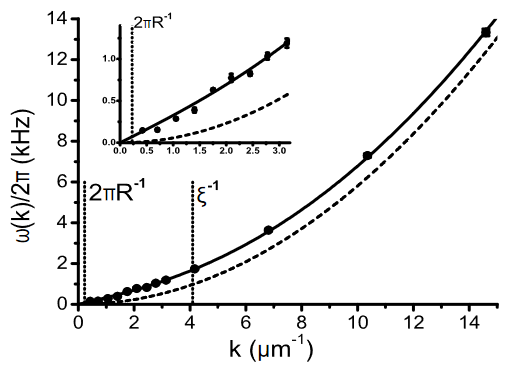
\includegraphics[width=0.65\textwidth]{Fig/Chapter1/bogo_steinhauer.png}
    \caption[Experimental observation of the Bogoliubov excitation spectrum]{Experimental observation of the Bogoliubov excitation spectrum (Steinhauer {\it et al.} \cite{steinhauer2002excitation}). The phononic and free particle parts are clearly identifiable. The inset shows a zoom on the linear part of the spectrum and the dashed line the free particle spectrum. $\xi$ is the healing length of the condensate.}
    \label{fig:my_label}
\end{figure}

\subsection{Many-body ground state and quantum depletion}

\label{sec:many_body_ground_state}

The Bogoliubov approach describes the excitations of the weakly-interacting Bose gas as non-interacting quasi-particles. These quasi-particles therefore behave as ideal bosons and are populated by the finite temperature with the Bose distribution:

\begin{equation}
    \langle b^{\dagger}_{\bm{k}}  b_{\bm{k}} \rangle=\frac{1}{e^{\varepsilon(k)/(k_B T)}-1} 
    \label{eq:bose_qp}
\end{equation}

\noindent At $T=0$, the population of quasi-particles is null: $\langle \hat{b}^{\dagger}_{\bm{k}}  \hat{b}_{\bm{k}} \rangle_{T=0}=0$. What can we say about real particles? By using the Bogoliubov transform, one can express the population of particles for a given momentum $k \neq 0$:

\begin{equation}
    \langle \hat{a}^{\dagger}_{\bm{k}}  \hat{a}_{\bm{k}} \rangle=\textcolor{blue}{(|u_k|^2+|v_k|^2)\langle \hat{b}^{\dagger}_{\bm{k}}  \hat{b}_{\bm{k}} \rangle} + \textcolor{green}{|v_k|^2}
\end{equation}

\noindent The blue term corresponds to the Bogoliubov excitations populated by temperature. The fraction of particles removed from the condensate this way is called the \textcolor{blue}{\textbf{thermal depletion}}. This fraction vanishes at $T=0$. Interestingly, an additional term \textcolor{green}{$|v_k|^2$} is present that results from the non commutation of the bosonic creation and annihilation operators, the signature of an essentially quantum phenomenon. This term implies that $\langle \hat{a}^{\dagger}_{\bm{k}}  \hat{a}_{\bm{k}} \rangle_{T=0} \neq 0$, meaning that there is a fraction of atoms outside of the BEC with a non zero momentum in the ground state! Under the interplay between interactions and quantum fluctuations, some atoms are removed from the BEC and promoted to non zero momentum states. This fraction is called the \textcolor{green}{\textbf{quantum depletion}}. 


\subsection{Pairing mechanism in the quantum depletion}

\label{sec:pairing_mechanism}

We now look to build a microscopical, physically meaningful picture of how the quantum depletion emerges. We remind that a key ingredient of the Bogoliubov theory is that the only considered interaction processes are the ones involving two particles of the BEC or two particles outside of the BEC being brought into it. From this consideration, we understand that the atoms belonging to the quantum depletion were initially in the BEC and were removed from it after undergoing a two-body interaction process. The interaction process populating the quantum depletion thus involves two atoms in the BEC with a momentum value $k \simeq 0$. To conserve the overall momentum, the two atoms leaving the BEC then have opposite momenta $\bm{k}$ and $-\bm{k}$ and form a momentum correlated pair. This falls exactly into the kind of signal we are interested in, namely correlations between several particles, here two, caused by a quantum, interaction-induced effect.

\begin{figure}
    \centering
    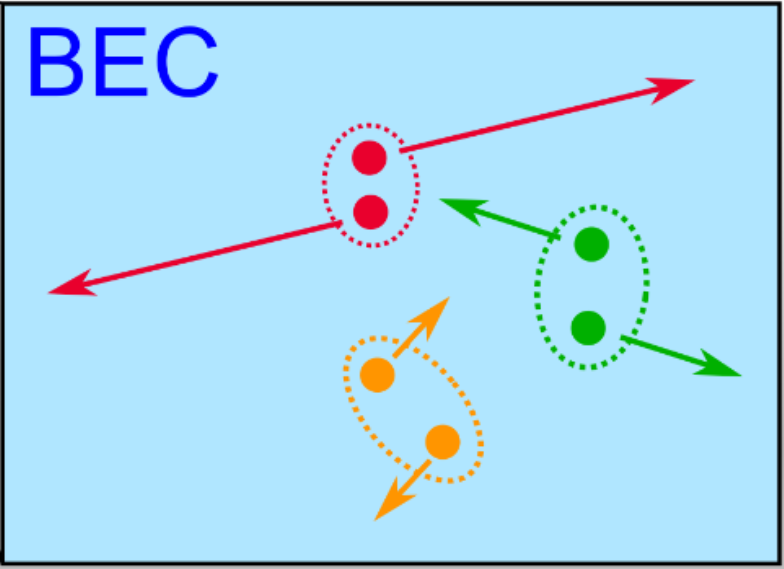
\includegraphics[width=0.5\textwidth]{Fig/Chapter1/pairs.png}
    \caption[Illustration of the \kmk pairing of the quantum depleted atoms in the BEC]{Illustration of the \kmk pairing of the quantum depleted atoms in the BEC (light blue).}
    \label{fig:bec_pairs}
\end{figure}

The common factor with quantum effects is that they usually defy our intuition built on our observation of the everyday world, well described by classical physics. In this case, the ``quantum weirdness'' comes from the fact this process seems to violate the conservation of energy. Initially, the two atoms belong to the \textbf{at-rest} BEC, their total kinetic energy is then zero. After the collision process, they acquire momenta $\bm{k}$ and $-\bm{k}$ meaning that the total kinetic energy is $2 (\hbar^2 k^2/2m) \neq 0$. Naturally, the conservation of energy is still well respected here. The apparent contradiction comes from the fact that it is conceptually wrong to isolate two atoms in the BEC. Every atom of the ground state belongs to the same quantum state, which exhibits non zero momentum components at large momenta. Because the pairs are created by the interaction term of the Hamiltonian, the pair creation is a coherent process. The many-body ground state is thus a superposition of the BEC and the pairs and writes:

\begin{equation}
     \ket{\psi_B} \sim \exp \Big(\sqrt{N_0} a^{\dagger}_0 + \sum_{\bm{k} \neq 0} (v_k/u_k) a^{\dagger}_{-\bm{k}} a^{\dagger}_{\bm{k}} \Big) \ket{0}
     \label{eq:ground_state}
\end{equation}

\noindent which is of the same form of the ground-state of the Bardeen-Cooper-Schrieffer theory of supraconductivity \cite{bardeen1957theory}. 

The energy of the many-body ground state of the weakly-interacting Bose gas thus contains a small correction that corresponds to the presence of the \kmk pairs of the quantum depletion. This small correction is called the Lee-Huang-Yang correction, named after the authors of the seminal 1957 article \cite{lee1957} that first predicted the presence of the \kmk pairs. 

%While there have already been experimental studies confirming the presence of quantum depleted atoms with large momentum \cite{sokol1995,xu2006} and the prediction of the quantum depleted fraction \cite{lopes2017}, the \kmk correlations in the ground-state have not yet been observed.

This pairing effect is quite reminiscent of the spontaneous parametric down conversion photon pairing effect that we saw in \ref{sec:amp_parametric}. The analogy between the non-degenerate parametric amplifier and the Bogoliubov Hamiltonian, replacing modes 1 and 2 by modes $\bm{k}$ and $-\bm{k}$ will in fact allow us to re-use the majority of the results derived in \ref{sec:amp_parametric} for the \kmk pairs. There is however one crucial difference, which is that the non-degenerate parametric amplifier is an \textbf{out-of-equilibrium}, \textbf{time-dependent} problem contrary to the \textbf{equilibrium} weakly-interacting Bose gas. This is in fact the fascinating aspect of the \kmk pairs of the quantum depletion whose existence can only be explained by the effect of quantum fluctuations.


% Although we cannot draw a rigorous direct analogy, this kind of effect is reminiscent of other puzzling phenomenon such as Hawking radiation \cite{hawking1974} describing the evaporation of black holes where a pair of correlated photons is produced near the event horizon, or the creation of particle/anti-particle pairs from the vacuum. By studying this \kmk correlation signal, we can therefore study how quantum correlations and possibly entanglement emerges in at-equilibrium quantum many-body systems from the interplay between quantum fluctuations and interactions, which constitutes an exciting prospect that will be the principal motivation of this thesis.

We are thus looking at a system which falls into our general area of interest described in the introduction of this thesis, namely many-body systems with interactions displaying quantum behaviors. The weakly-interacting Bose gas shows the advantage to be one of the conceptually simplest many-body systems for which a theory can be derived as we just have shown. We will now build a bridge with the first part of this chapter by discussing what are the relevant correlation functions to study the weakly-interacting Bose gas.


\section{Two-body correlations in the homogeneous weakly-interacting Bose gas}

% \subsection{Second order correlation functions within Bogoliubov theory}

\label{sec:2nd_order_bogo}

Now that we have identified the \kmk pairing mechanism in the quantum depletion, it is natural to look for a signature of it in the second order correlation function that characterizes the correlations between two particles \cite{butera2020,mathey2009noise,toth2008theory}. We start by describing the general case of the two-body correlator between two modes $\bm{k}$ and $\bm{k'}$:

\begin{equation}
    G(\bm{k},\bm{k}')=\langle \hat{a}^{\dagger}_{\bm{k}} \hat{a}^{\dagger}_{\bm k'} \hat{a}_{\bm k} \hat{a}_{\bm {k}'} \rangle
\end{equation}

As we have seen in the previous section, the Bogoliubov Hamiltonian is diagonal in the quasi-particle basis, meaning that all quantum states have Gaussian statistics in this basis. As the Bogoliubov transformation is linear and therefore conserves Gaussianity, the statistics are Gaussian in the particle basis as well \cite{butera2020}. We can the apply Wick's theorem (see \ref{sec:wick}) to simplify the correlator:

\begin{equation}
    G(\bm{k},\bm{k}')=\langle \hat{a}^{\dagger}_{\bm k} \hat{a}^{\dagger}_{\bm {k}'} \rangle \mean{\hat{a}_{\bm k} \hat{a}_{\bm {k}'}} + \langle \hat{a}^{\dagger}_{\bm k} \hat{a}_{\bm k} \rangle \langle \hat{a}^{\dagger}_{\bm {k}'} \hat{a}_{\bm {k}'} \rangle + \langle \hat{a}^{\dagger}_{\bm k} \hat{a}_{\bm {k}'} \rangle \langle \hat{a}^{\dagger}_{\bm {k}'} \hat{a}_{\bm k} \rangle
    \label{eq:wick_bogo}
\end{equation}

We end up with three different terms:

\begin{itemize}
    \item The first term that equals $| \langle \hat{a}^{\dagger}_{\bm k} \hat{a}^{\dagger}_{\bm {k}'} \rangle |^2$.
    \item We recognize in the second term the product of the momentum densities $\rho(\bm{k}) \rho(\bm{k}')$.
    \item The third term that equals $| \langle \hat{a}^{\dagger}_{\bm k} \hat{a}_{\bm {k}'} \rangle |^2$. 
\end{itemize}

\noindent We regroup the two last terms in the function $G^{(2)}_{N}({\bm k},{\bm k}')= \rho({\bm k})\rho({\bm k}') + | \langle \hat{a}^{\dagger}_{\bm k} \hat{a}_{\bm {k}'} \rangle |^2$ that we call the \textbf{normal} correlation function as the operators are normally ordered (see \ref{sec:normal_order}). In opposition, we introduce for the last term the function $G^{(2)}_{A}({\bm k},{\bm k}')=| \langle \hat{a}^{\dagger}_{\bm k} \hat{a}^{\dagger}_{\bm {k}'} \rangle |^2 $ that we call the \textbf{anomalous} correlation function. Interestingly, this term is non zero only if there exists interactions coupling different modes, in our case $\bm{k}$ and $-\bm{k}$.

We must now determine which atoms participate to which correlation signal. We have seen in \ref{sec:many_body_ground_state} that the depletion of the condensate is divided between the \textbf{quantum} and the \textbf{thermal} depletion. As we have shown in \ref{sec:pairing_mechanism}, we expect that the quantum depleted atoms contribute to the anomalous \kmk correlation signal due to the microscopic mechanism describing how the quantum depletion is populated. In fact, it is also possible for the thermal depletion to contribute to the anomalous correlation signal. Indeed, as discussed in \ref{sec:spectrum}, for low $k$ values such as $k \xi \ll 1$, the Bogoliubov quasi-particles have a strong phononic character $\hat{b}_{\bm{k}}=u_{\bm{k}} \hat{a}_{\bm{k}} + v_{-\bm{k}} \hat{a}^{\dagger}_{-\bm{k}}$ with $\abs{u_{\bm{k}}} \simeq \abs{v_{-\bm{k}}}$ and exhibits non negligible \kmk correlations. This is an issue as if we were to observe \kmk correlations, we would not be able to unambiguously attribute them to the quantum depletion as they could come from phonons of the thermal depletion. To quantify this contribution, we use Bogoliubov's transformation to rewrite equation \ref{eq:wick_bogo} in its normalized form in terms of quasi-particle operators and Bogoliubov coefficients $u_k$ and $v_k$ \cite{butera2020,mathey2009noise}.

\begin{equation}
    \gtwo (\bm{k},\bm{k}') = \frac{| u_k v_k (1+2\langle \hat{b}^{\dagger}_{\bm{k}} \hat{b}_{\bm{k}} \rangle)| ^2 }{\Big((|u_k|^2+|v_k|^2)\langle \hat{b}^{\dagger}_{\bm{k}}  \hat{b}_{\bm{k}} \rangle + |v_k|^2 \Big)^2} \delta_{\bm{k},\bm{-k'}}+ \delta_{\bm{k},\bm{k}'} + 1
    \label{eq:g2_uv}
\end{equation}




\begin{figure}
    \centering
    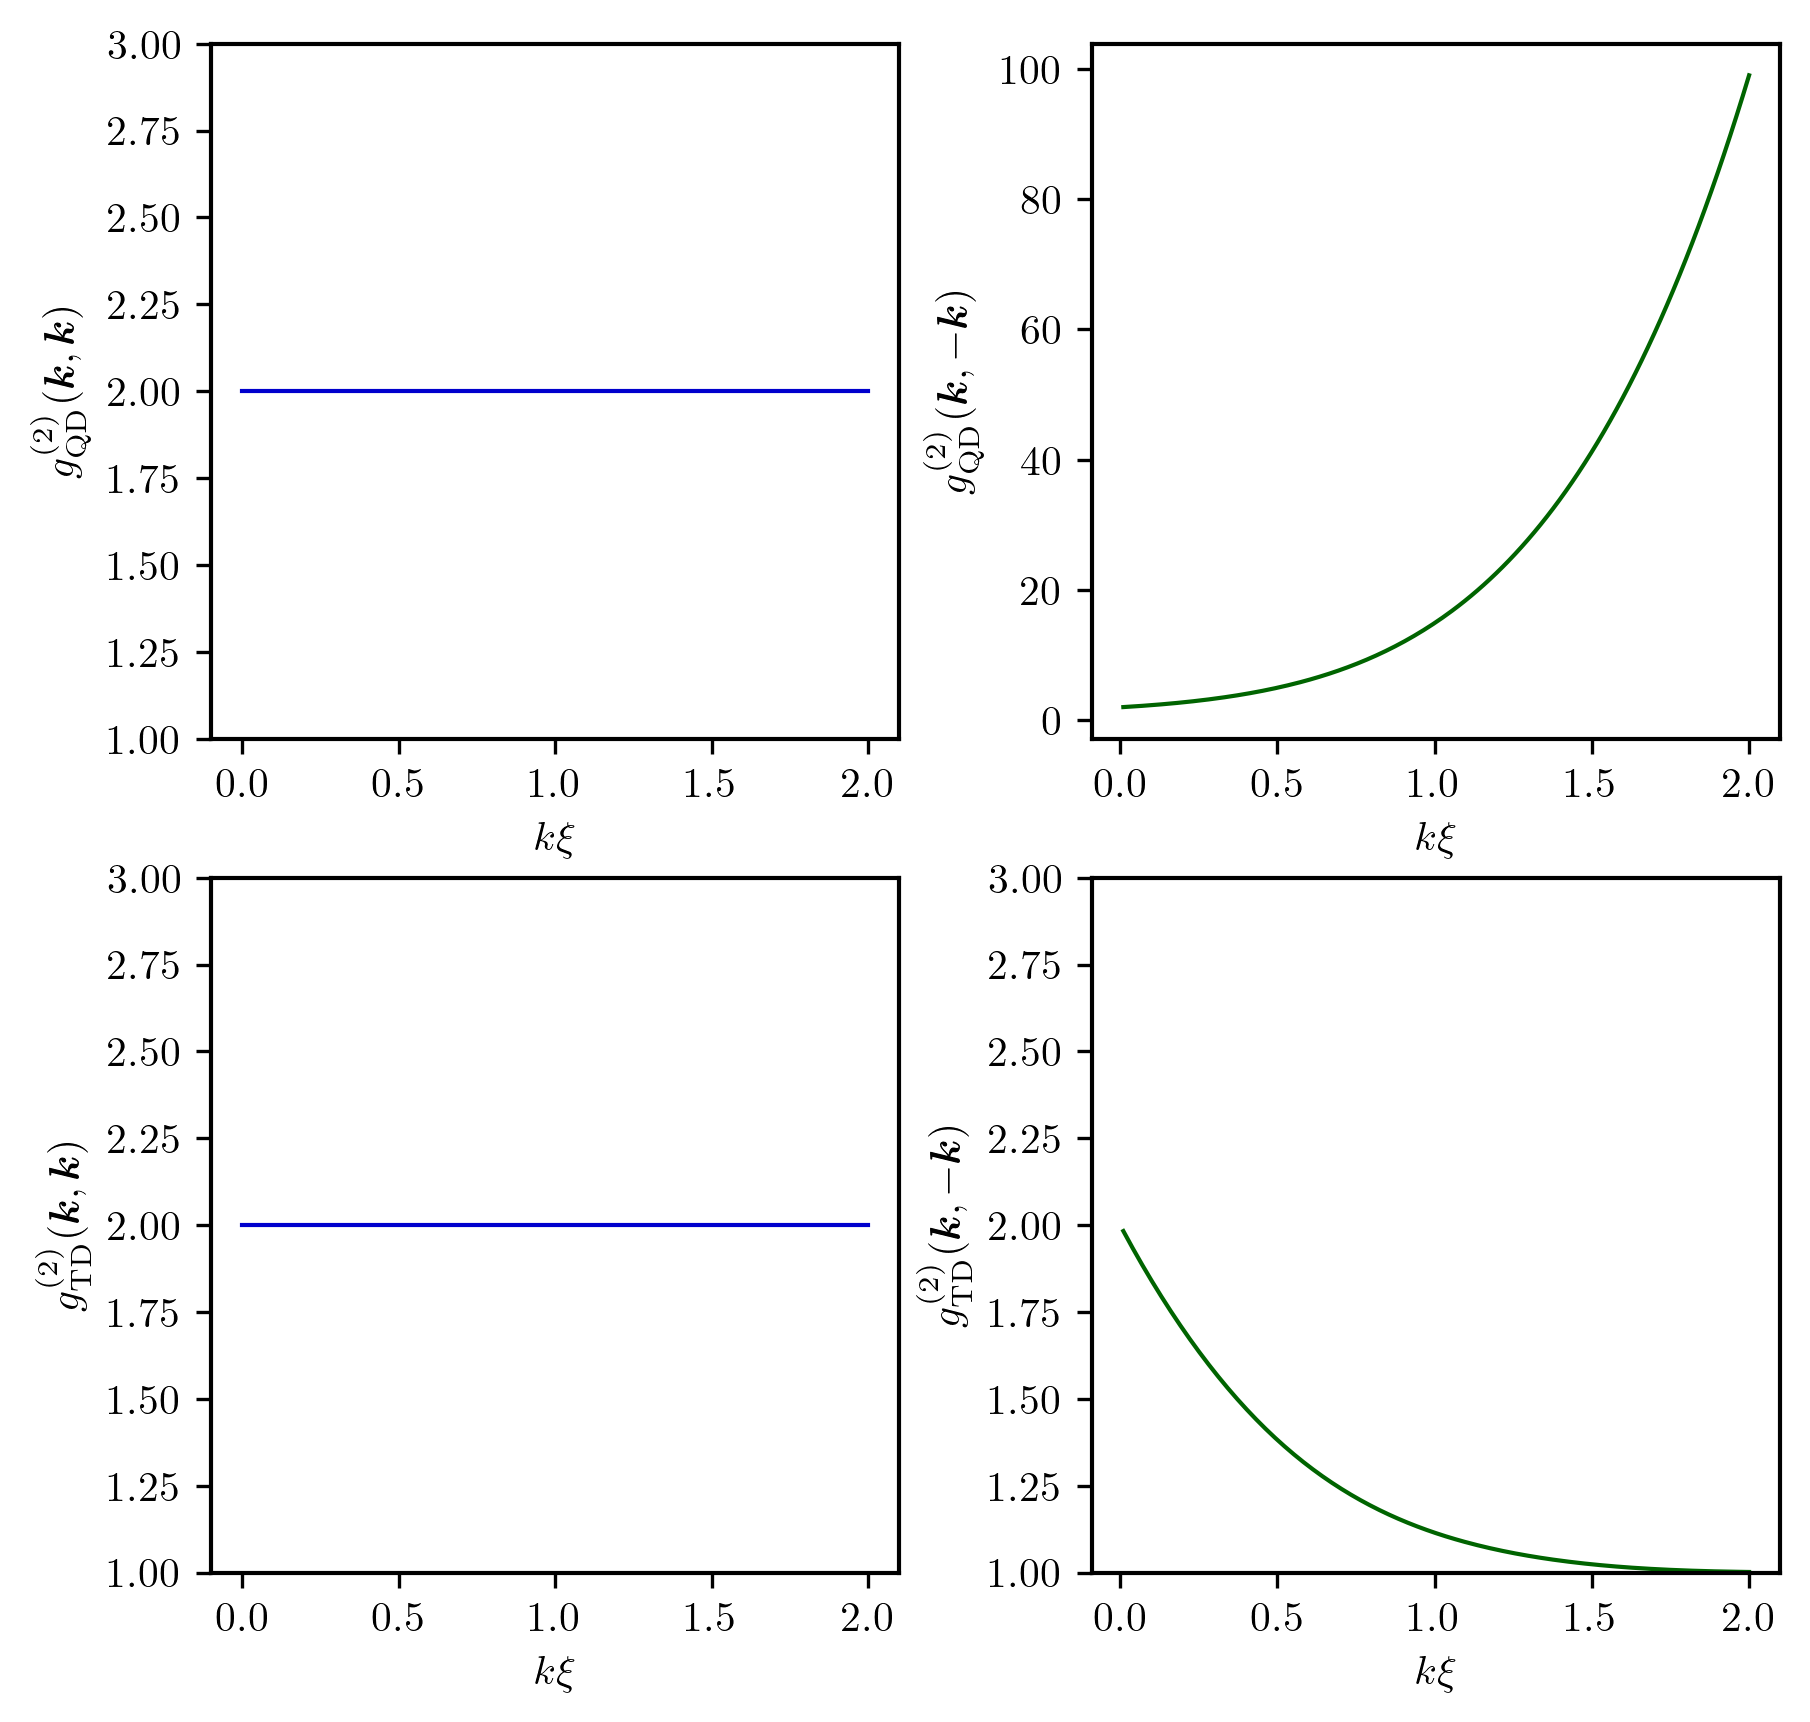
\includegraphics[width=\textwidth]{Fig/Chapter1/g2_bogo.png}
    \caption[Second order correlation function for normal \kk correlations and anomalous \kmk correlations with quantum and thermally depleted atoms]{Second order correlation function for normal \kk correlations (blue) and anomalous \kmk correlations (green) with quantum (subscript QD) and thermally depleted (subscript TD) atoms (resp. top and bottom row) as a function of $k \xi$. These results are obtained from the Bogoliubov theory of the weakly-interacting, homogeneous, 1D Bose gas with a chemical potential $\mu/h=1.5 \ \rm{kHz}$ and temperature $T=60 \ \rm{nK}$.}
    \label{fig:g2_bogo}
\end{figure}

The function $\gtwo (\bm{k},-\bm{k})$ is plotted on Fig.-\ref{fig:g2_bogo} for both quantum ($T=0$) and thermally depleted atoms. As $k \xi$ increase, the density of quantum depleted atoms decreases, meaning 
that their contribution to $\gtwo (\bm{k},-\bm{k})$ increases following from the analogy with the the non-degenerate parametric amplifier and the result of equation \ref{eq:amp_g2_A}. On the contrary, the contribution of the thermally depleted atoms decreases with $k \xi$ as the phononic character of the quasi-particles disappears, and becomes negligible for $k \xi \leq 1$. This gives us a nice workaround: if we restrict our measurement of \kmk correlations to large $k$, we could safely attribute them to the quantum depletion.

Let us now take a look at normal correlations, \ie bosonic bunching. We get from equation \ref{eq:g2_uv} and the plots of Fig.-\ref{fig:g2_bogo} that we have perfect bosonic bunching independently of $k$ for both quantum and thermally depleted atoms. As we have seen in \ref{sec:spectrum} and \ref{sec:many_body_ground_state}, the Bogoliubov quasi-particles of the thermal depletion follow the Bose distribution and therefore have thermal chaotic statistics, explaining the presence of bosonic bunching. On the other hand, the \kmk pairs of the quantum depletion form a pure coherent state (see equation \ref{eq:ground_state}) for which we would then not expect bosonic bunching as explained in \ref{sec:coherent_g2}. The situation is however a bit more subtle than that. In direct analogy with the non-degenerate parametric amplifier, when we look for same mode \kk correlations, we do so between atoms belonging to two different pairs. We retrieve a density matrix with a chaotic character \cite{yurke1987} by tracing over the second atom of the pair that we ignore, as proven in \ref{sec:amp_parametric}. This means that we should observe bosonic bunching with the quantum depletion as well \cite{butera2020}!

% Nonetheless, this low $k$ region corresponds more or less to the region that will need to be removed to exclude the BEC from the analysis (experimental numbers will be given in Chapter 4). We therefore do not have to care for the contribution of the thermal depletion to the \kmk correlation signal that will in our case only reflect the quantum depletion correlations.

In a nutshell, we have two correlation features of interest well separated in momentum space and containing very different types of information. On the one hand, the normal correlations correspond to close-by correlations and bosonic bunching revealing the chaotic statistics of the system, coming from either the thermal statistics of the thermal depletion, or the partial trace over the second atom of the pair destroying the quantum coherence for the quantum depletion. On the other hand, the anomalous correlations correspond to \kmk correlations and reveal the quantum coherences of the many-body ground state, provided that we probe them in the region $k \xi \geq 1$. While our main goal will be to measure the anomalous \kmk correlations for the reasons mentioned earlier, it will also be of great interest to measure the normal correlations to contrast their behaviour with the anomalous correlations as a means to illustrate the different physical origins of the two signals. 


% \subsection{Violation of the Cauchy-Schwarz inequality and Busch-Parentani criterion}

% \label{sec:cs_inequality}

% The very famous Cauchy-Schwarz inequality has seen countless applications in mathematics and physics. What will most interest us here is its formulation in the framework of probability theory. In classical physics, with two fluctuating quantities $I_1$ and $I_2$, the Cauchy-Schwarz inequality writes:

% \begin{equation}
%     \mean{I_1 I_2} \leq \sqrt{\mean{I_1^2} \mean{I_2^2}}
% \end{equation}

% This inequality can be rewritten with creation/annihilation operators to work with two-body correlation functions. Let us illustrate it with the simple case of two modes, those of the non-degenerate parametric amplifier or the momentum modes $\bm{k}$ and $-\bm{k}$ that we label as 1 and 2. We introduce the notation $G^{(2)}_{i,j} = \mean{\hat{a}_i^{\dagger} \hat{a}_j^{\dagger} \hat{a}_i \hat{a}_j}$. The Cauchy-Schwarz inequality becomes \cite{kheruntsyan2012violation,walls2008}:

% \begin{equation}
%     G^{(2)}_{1,2} \leq \sqrt{G^{(2)}_{1,1} G^{(2)}_{2,2} }
% \end{equation}

% In the symmetrical case with $\mean{\hat{a}^{\dagger}_1 \hat{a}_1}=\mean{\hat{a}^{\dagger}_2 \hat{a}_2}$ (true for both the non-degenerate parametric amplifier and \kmk correlations in the quantum depletion), we obtain $G^{(2)}_{1,1}=G^{(2)}_{2,2}$ and finally:

% \begin{equation}
%     \gtwo_A (1,2) \leq \gtwo_N (1,1)
% \end{equation}


% Therefore, the Cauchy-Schwarz inequality states that the cross-correlation amplitude cannot exceed the amplitude of the auto-correlation with a classical model. The result of equation \ref{eq:amp_g2_A} violates this inequality and is therefore the signature of a quantum phenomenon. As developed in \cite{kheruntsyan2012violation}, observing a violating the Cauchy-Schwarz inequality is one of the easiest way to prove the presence of non-classical correlations.

% In fact, violating the Cauchy-Schwarz inequality can be enough to demonstrate entanglement in some situations. The work \cite{busch2014quantum} devises the Busch-Parentani criterion for a state to be entangled that writes (switching back to the notations of Bogoliubov theory):

% \begin{equation}
%     \rho(\bm{k}) \rho(-\bm{k}) - | \langle \hat{a}^{\dagger}_{\bm k} \hat{a}^{\dagger}_{-\bm {k}} \rangle |^2 < 0
%     \label{eq:busch-parentani}
% \end{equation}

% \noindent From equation \ref{eq:wick_bogo}, we get

% \begin{equation}
%     \langle \hat{a}^{\dagger}_{\bm{k}} \hat{a}^{\dagger}_{-\bm k} \hat{a}_{\bm k} \hat{a}_{-\bm {k}} \rangle = | \langle \hat{a}^{\dagger}_{\bm k} \hat{a}^{\dagger}_{-\bm {k}} \rangle |^2 + \rho(\bm{k}) \rho(-\bm{k}) + \langle \hat{a}^{\dagger}_{\bm k} \hat{a}_{-\bm {k}} \rangle \langle \hat{a}^{\dagger}_{-\bm {k}} \hat{a}_{\bm k} \rangle
% \end{equation}

% \noindent where the last term is zero in Bogoliubov's theory. Injecting \ref{eq:busch-parentani}, we get:

% \begin{equation}
%     \langle \hat{a}^{\dagger}_{\bm{k}} \hat{a}^{\dagger}_{-\bm k} \hat{a}_{\bm k} \hat{a}_{-\bm {k}} \rangle > 2 \rho(\bm{k}) \rho(-\bm{k})
% \end{equation}

% \noindent Dividing by  $\rho(\bm{k}) \rho(-\bm{k})$, we obtain:

% \begin{equation}
%     \gtwo_A (\bm{k},-\bm{k}) > 2 \Longleftrightarrow \gtwo_A (\bm{k},-\bm{k}) > \gtwo_N (\bm{k},\bm{k})
% \end{equation}

% \noindent which is strictly equivalent to violating the Cauchy-Schwarz inequality. Note that this development holds only if \textit{(i)} the statistics of the system are chaotic so that we can apply Wick's theorem and have $\gtwo_N (\bm{k},\bm{k})=2$, \textit{(ii)} $\langle \hat{a}^{\dagger}_{\bm k} \hat{a}_{-\bm {k}} \rangle \langle \hat{a}^{\dagger}_{-\bm {k}} \hat{a}_{\bm k} \rangle=0$ which is true in Bogoliubov's theory but needs experimental proof if we wish to claim experimental observation of entanglement in momentum space.
  
\section{Effects of an external trapping potential}

\label{sec:width_correlation_theo}
  
The weakly-interacting \textbf{homogeneous} Bose gas Hamiltonian does not actually faithfully represent our experiment as we use an external harmonic potential $V(\bm{r})$ to trap the atoms, making the system not homogeneous anymore. This makes the theoretical approach significantly more difficult, but still manageable through numerical calculations as it was recently done in \cite{butera2020} to evaluate the correlation functions in the trapped case.

In this section, we will summarize the main results of \cite{butera2020} to show how the spatial size of the system affects the widths of the correlation signals and obtain estimates for comparison with experimental data. Indeed, as we have seen in the Hanbury Brown and Twiss experiment aiming to measure the size of Sirius through the measurement of the second order correlation function, the width of the correlation function is inversely proportional to the spatial size of the source. 

\subsection{Normal correlations}

\label{sec:width_normal_theo}

As discussed in the last paragraph for the homogeneous case, we expect a perfect bosonic bunching $g^{(2)}(\bm{k},\bm{k})=2$ for both the thermal and the quantum depletion. This feature is actually the same in the trapped case as shown in \cite{butera2020} where the numerical calculations also give a perfect bosonic bunching, independently of the temperature and thus of the balance between the thermally and quantum depleted atoms. The width of the correlation peak shows however quite interesting dependencies on the momentum value $k$ and the temperature.

At $T=0$ or very low temperatures, the RMS width $\sigma_k$ of the normal correlations is dominated by the contribution of the quantum depletion. As the quantum depletion is non-existent outside of the BEC, its spatial size is the one of the BEC, meaning that the width of the normal correlations at $T=0$ should be $\sim 1/L_{\rm{BEC}}$ with $L_{\rm{BEC}}$ the spatial size of the BEC, and so independently of $k$. This is what we observe on Fig.-\ref{fig:butera_kk} from \cite{butera2020}, with however a small increase of the width with $k$ that the authors attribute to a stronger localisation of the highly-excited Bogoliubov modes associated to the quantum depletion.
For $T \neq 0$ however, the dependency of the normal correlations width with $k$ is non-monotonic. At large $k$, we retrieve the same width than for $T=0$. Indeed, the thermal energy is not sufficient to populate such high $k$ values. The depletion is thus fully quantum and the width $\sim 1/L_{\rm{BEC}}$. As $k$ decreases, we progressively reach a momentum region where the depletion is mainly thermal. As the spatial size of the thermal excitations is larger than that of the BEC because of the increased kinetic energy, $\sigma_k$ is reduced. We then enter a plateau region that starts for higher values of $k$ and stabilizes around lower values of $\sigma_k$ as $T$ increases as shown on Fig.-\ref{fig:butera_kk}. The plateau region ends for very low values of $k$ as $\sigma_k$ slightly increases with decreasing $k$ that the authors of \cite{butera2020} attribute to the phononic character of the thermal excitations in this $k$ region.


\begin{figure}
    \centering
    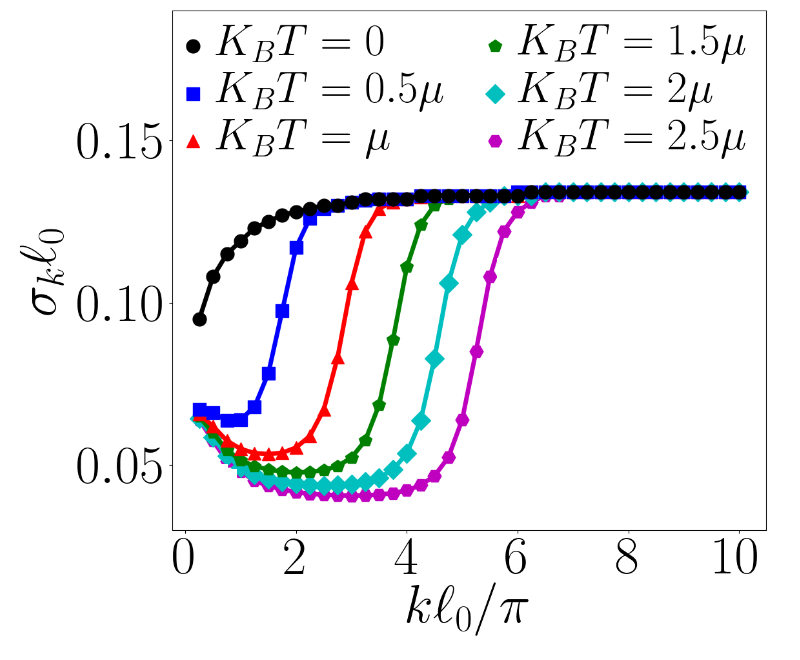
\includegraphics[width=0.6\textwidth]{Fig/Chapter1/butera.png}
    \caption[Evolution of normal correlations width with $k$ for different values of the temperature]{Evolution of the normal correlations width $\sigma_k l_0$ as a function of $k l_0/\pi$ with $l_0=\sqrt{\hbar/2m \omega}$ where $\omega$ is the trapping frequency for different values of the temperature. Taken from \cite{butera2020}.}
    \label{fig:butera_kk}
\end{figure}

% To properly understand the situation, we will compare the predictions for both anomalous and normal correlations. We then need to determine what are the sizes of the components responsible for both correlation signals. On the one hand, the anomalous correlations are exclusively caused by quantum depleted atoms. The quantum depletion is non-existent outside of the BEC so its spatial is the one of the BEC. Therefore, we expect the width of the anomalous correlation peak $\sigma_A$ to be inversely proportional to the size of the BEC $L_{\rm{BEC}}$. On the other hand, the normal correlations are caused by quantum depleted atoms but also and importantly thermally depleted atoms whose spatial size extends beyond the BEC because of the increased kinetic energy. This tells us that the width of the normal correlations peak $\sigma_N$ should be smaller than for anomalous correlations.

\subsection{Anomalous correlations}

\label{sec:width_anomalous_theo}

The situation is more straightforward for the anomalous correlations related to the quantum depletion that is not affected by the temperature. The width of the anomalous correlations is therefore almost insensitive to temperature and independent from $k$, apart from a small increase at low $k$ in the same fashion than for normal correlations at $T=0$ (see Fig.-\ref{fig:butera_kmk}). 

\begin{figure}
    \centering
    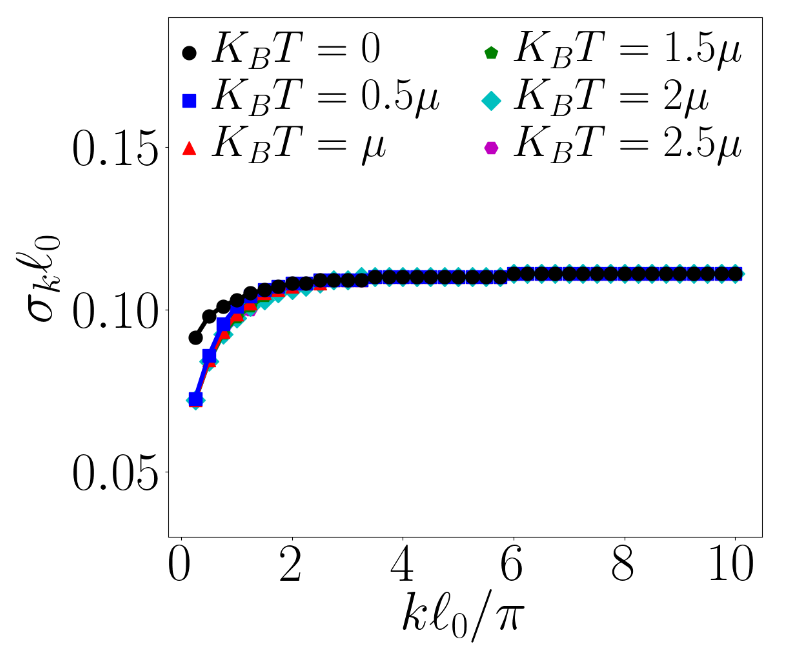
\includegraphics[width=0.6\textwidth]{Fig/Chapter1/butera_kmk.png}
    \caption[Evolution of the anomalous correlations width with $k$ for different values of the temperature]{Evolution of the anomalous correlations width $\sigma_k l_0$ as a function of $k l_0/\pi$ for different values of the temperature. Taken from \cite{butera2020}.}
    \label{fig:butera_kmk}
\end{figure}

\section{Towards the experimental detection of k/-k pairs}

Now that we have formed a clear picture of the kind of correlation functions we want to measure and have understood their essential features, we need to identify the key experimental ingredients necessary to observe such signals. The principal one is to have an experiment capable of measuring the momentum of individual atoms in momentum space and not only the momentum density as in most cold atoms experiment. This will be the subject of Chapter \ref{sec:chapter_3}. 

In addition, there are several key features of the \kmk correlation signal that we need to understand to design an experimental scheme where the \kmk correlation signal can be properly detected.


\subsection{Separating the BEC from its depletion}

\label{sec:ch1_separation}

A crucial aspect of studying the correlations in the depletion is the ability to separate the depleted atoms from the condensed ones. As a matter of fact, the BEC is a fully coherent state with macroscopic occupation of a single mode. In analogy with laser light in Optics, the statistics of the BEC are not chaotic and no bosonic bunching can therefore be observed. In addition, no \kmk correlations are expected for atoms belonging to the condensate. Furthermore, in the weakly-interacting BEC, the number of condensed atoms is much larger than the number of depleted atoms. This has a direct consequence for our measurement: if we are unable to remove condensed atoms from the analysis, they will entirely drown out the correlation signals of the depletion.

Fortunately, the BEC and the depletion extents in momentum space are very different. As for the width of the first-order correlation functions, the typical size of the momentum mode of the BEC is $1/L_{\rm{BEC}}$ \cite{stenger1999}. On the other hand, the typical momentum width of the quantum depletion is $1/\xi$. Since $\xi \ll L_{\rm{BEC}}$, $1/\xi \gg 1/L_{\rm{BEC}}$ meaning that the quantum depletion extends on a much larger momentum area than the BEC. Likewise, for the typical temperatures accessible in our experiment, the momentum width of the thermal depletion is significantly larger than for the BEC.
This effect is illustrated on Fig.-\ref{fig:density_lattice_ch1}. This provides us with a natural way to separate the condensate from its depletion and defines one of the experimental ingredients: we need an experimental setup capable of resolving the different regions of momentum space so that the region around $\bm{k}=\bm{0}$ corresponding to the BEC can be removed from the analysis. In addition, while removing the BEC region we also remove the low $k$ part of the momentum space in which the Bogoliubov quasi-particles have a strong phononic character (see Chapter \ref{sec:chapter_4} for experimental numbers) and thus \kmk correlations between particles, fulfilling the requirement described in \ref{sec:2nd_order_bogo}.



\begin{figure}
    \centering
    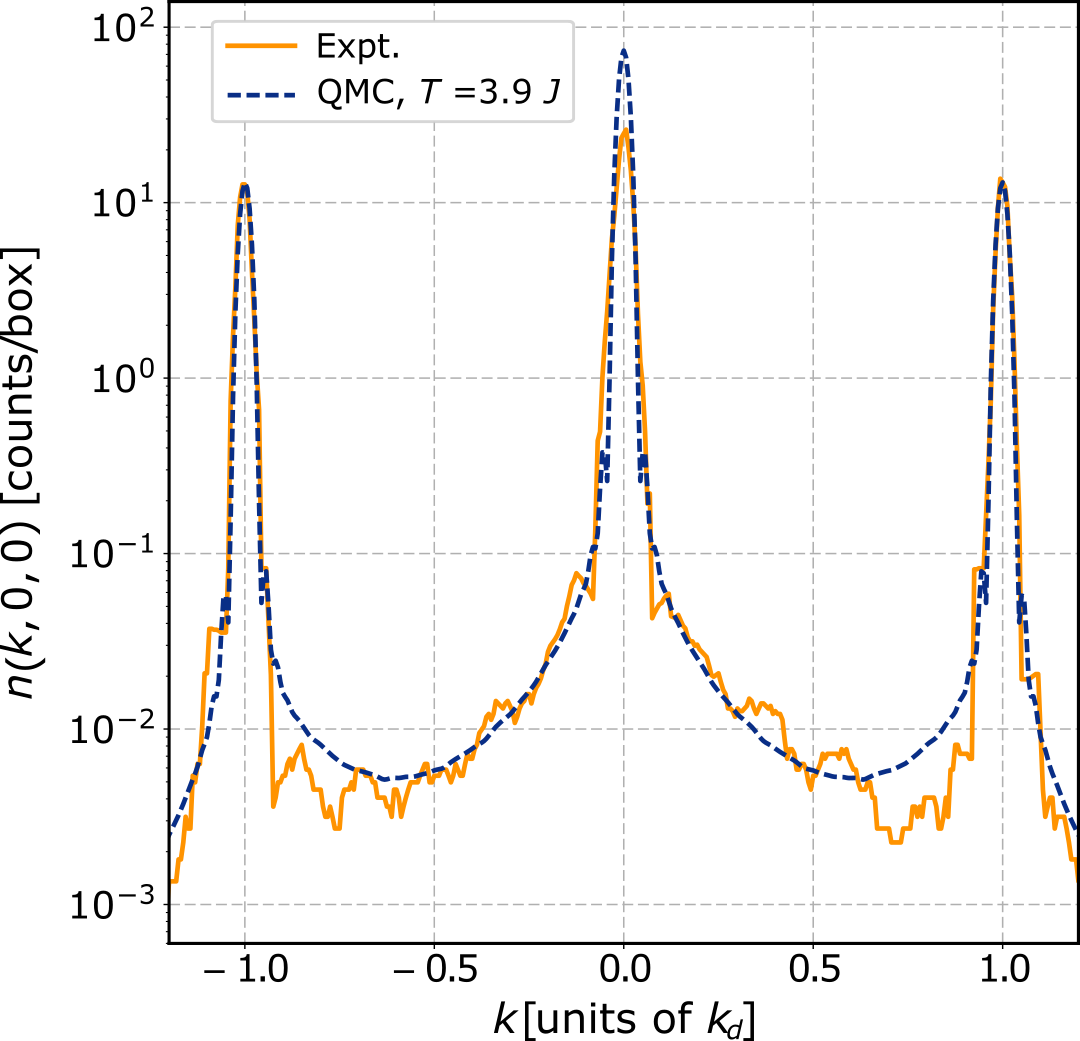
\includegraphics[width=0.6\textwidth]{Fig/Chapter1/cayla_2018.png}
    \caption[Illustration of the different momentum extents of the BEC and the depletion]{Experimental momentum density illustrating the different momentum extents of the BEC and the depletion. The condensed atoms correspond to the sharp and narrow peaks, as opposed to the wide background between the peaks that correspond the depletion. Note that the presence of several condensed peaks is linked to the presence of an optical lattice, as it will be explained in Chapter \ref{sec:chapter_2}. Taken from \cite{cayla2018single}.}
    \label{fig:density_lattice_ch1}
\end{figure}


\subsection{Finite temperature effects}

\label{sec:ch1_temperature}

Another parameter that we must be very careful of is the temperature. In an ideal situation, we would conduct the experiment at zero temperature where the depletion is entirely quantum and all atoms consequently \kmk paired. Obviously this is impossible to do in practice and the experiment will always be conducted at finite temperature.

Temperature is an absolutely crucial parameter when measuring \kmk correlations as it sets the population of the thermal depletion, {\it i.e.} the population of the Bogoliubov quasi-particles (see equation \ref{eq:bose_qp}). Indeed, as we have just seen, thermally depleted atoms show no \kmk correlations in the momentum range that we wish to probe. If the temperature is too high, the thermally depleted atoms will significantly outnumber the quantum depleted ones and it will then be impossible to detect the \kmk correlations. In order to quantify the effect of temperature, we compare the typical thermal energy $k_B T$ to the chemical potential of the condensate $\mu$ quantifying the effect of interactions. We aim to be in an experimental regime where $k_B T \ll \mu$, {\it i.e.} where interactions effects dominate temperature effect. The first idea that comes to mind is then to reduce the temperature as much as possible. We however quickly hit a brick wall: the lowest temperature in ultracold experiments are obtained through evaporative cooling. This process will be detailed in Chapter \ref{sec:chapter_3} but we can quickly give here the main idea, which is to selectively remove the atoms of the gas with the highest thermal energy to let the other thermalize at a colder temperature. We quickly see the problem here: when the energy is dominated by the interaction energy $\sim \mu$ with $\mu$ the chemical potential, the atoms are removed randomly with respect to their thermal energy and there is thus no cooling anymore. This method allows us to typically reach $k_B T \sim 0.75 \mu$ \cite{chang2016} which is not sufficient to ensure the proper detection of \kmk correlations.

We are thus left with one only possible solution which is to increase the interactions. To this end, we will use a \textbf{3D optical lattice}. As a brief overview, a 3D optical lattice is formed by interference of 3 pairs of countra-propagating beams, one for each direction of space. The interferences create a sinusoidal potential trapping the atoms at the maximum of the light intensity profile, {\it i.e.} in periodically arranged wells, mimicking a condensed matter crystal. Interestingly, the density increases inside of the individual wells as a result of higher local trapping frequencies, increasing the strength of interactions and thus the likelihood to observe \kmk correlations.



\section{Conclusion}

In this chapter, we have shown that correlation functions are an important and powerful tool that was first developed to describe classical effects of the light such as interferences. The experiment of Hanbury Brown and Twiss introduced the use of second-order correlation functions and revealed the existence of bosonic bunching. This observation later gave birth to the Quantum Optics formalism and the extended theory of coherence developed by R. J. Glauber with higher order correlation functions. This formalism was then adapted to atomic physics where correlation functions are of great interest to characterize \textbf{many-body interacting} systems. We made the proposition to study one of the simplest many-body system, the weakly-interacting Bose gas described by the Bogoliubov theory that we detailed the main lines of. We have shown that the Bogoliubov theory predicts the existence of the quantum depletion, a fraction of atoms removed from the condensate through the interplay between interactions and quantum fluctuations, and that we expect these atoms to form \kmk correlated pairs that we will aim to detect by measuring second-order correlation functions. To this end, we have devised that our experimental setup should:

\begin{itemize}
    \item Detect single atoms in momentum space.
    \item Isolate the contribution of the depletion from the one of condensed atoms.
    \item Be in the low-temperature regime where interactions dominate temperature effects $k_B T \ll \mu $. 
\end{itemize}

We decided for this last point to use 3D optical lattices that we will discuss in details in the next chapter of this thesis.